\chapter{Deformations of Shannon entropy}
\lbl{ch:def}
\index{deformation}
\index{entropy!deformations of}

Shannon entropy is fundamental, but it is not the only useful or natural
notion of entropy, even in the context of a single probability distribution
on a finite set.  In this chapter, we meet two one-parameter families of
entropies that both include Shannon entropy as a member
(Figure~\ref{fig:defs}).
% 
\begin{figure}
\centering
\lengths
\begin{picture}(120,40)(7,-4)
% \graphpaper[2](7,-4)(120,40)
\cell{60}{20}{c}{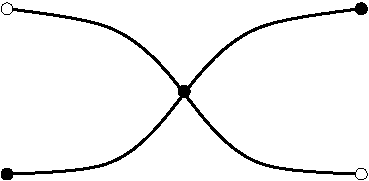
\includegraphics[height=30\unitlength]{defs}}
\cell{25}{34}{c}{$-\infty$}
\cell{25}{6}{c}{$-\infty$}
\cell{93}{34}{c}{$\infty$}
\cell{93}{6}{c}{$\infty$}
\cell{75}{28}{l}{R\'enyi entropies $H_q$}
\cell{75}{10}{l}{$q$-logarithmic entropies $S_q$}
\cell{60}{4}{b}{\vector(0,1){14}}
\cell{60}{0}{b}{Shannon entropy}
\cell{60}{-4}{b}{$H_1 = H = S_1$}
\end{picture}
\caption{Two families of deformations of Shannon entropy: the R\'enyi
  entropies $(H_q)_{q \in [-\infty, \infty]}$ and the $q$-logarithmic
  entropies $(S_q)_{q \in (-\infty, \infty)}$.}  
\lbl{fig:defs}
\end{figure}
% 
Both are indexed by a real parameter $q$, and both have Shannon entropy as
the case $q = 1$.  Moving the value of $q$ away from $1$ can be thought of
as deforming Shannon entropy.  As in other mathematical contexts where
the word `deformation' is used, the undeformed object (Shannon
entropy) has uniquely good properties that are lost after deformation,
but the deformed objects nevertheless retain some of the original object's
features.  

We begin with the $q$-logarithmic entropies $(S_q)_{q \in \R}$, often
called `Tsallis entropies' (a misattribution detailed in
Remark~\ref{rmk:q-log-ent-name}).  The $q$-logarithmic entropies have been
used as measures of biological diversity, but should probably not be, as we
will see (Examples~\ref{egs:q-ent}).

Perhaps surprisingly, it is \emph{easier} to uniquely characterize the
entropy $S_q$ for $q \neq 1$ than it is in the Shannon case $S_1 = H$.
Moreover, the characterization theorem that we prove does not require any
regularity conditions at all, not even measurability.  The same goes for
the $q$-logarithmic relative entropy, which we also introduce and
characterize. 

After some necessary preliminaries on the classical topic of power means
(Section~\ref{sec:pwr-mns}), we introduce the other main family of
deformations of Shannon entropy: the R\'enyi entropies $(H_q)_{q \in
  [-\infty, \infty]}$ (Section~\ref{sec:ren-hill}).  The
$q$-logarithmic and R\'enyi entropies have exactly the same content: for
each finite value of $q$, there is a simple formula for $S_q(\p)$ in terms
of $H_q(\p)$, and vice versa.  But they have different and complementary
algebraic properties.  For instance, the $q$-logarithmic entropies satisfy
a simple chain rule similar to that for Shannon entropy, whereas the chain
rule for the R\'enyi entropies is more cumbersome.  On the other hand,
the R\'enyi entropies have the same log-like property as Shannon
entropy, 
\[
H_q(\p \otimes \vc{r}) = H_q(\p) + H_q(\vc{r}),
\]
but the $q$-logarithmic entropies do not.

The exponential of R\'enyi entropy, $D_q(\p) = \exp(H_q(\p))$, is known in
ecology as the Hill number of order $q$.  The Hill numbers are the most
important measures of biological diversity (at least, if we are using the
crude model of a community as a probability distribution on the set of
species).  Different values of $q$ reflect different aspects of a
community's composition, and graphing $D_q(\p)$ against $q$ enables one to
read off meaningful features of the community.  In
Sections~\ref{sec:ren-hill} and~\ref{sec:prop-hill}, we illustrate this
point and establish the properties that make the Hill numbers so suitable
as measures of diversity.

We finish by showing that the Hill number of a given order $q$ is uniquely
characterized by certain properties (Section~\ref{sec:hill-char-given}).
The same is therefore true of the R\'enyi entropies (since one is the
exponential of the other), although the properties appear more natural when
stated for the Hill numbers.  This is the first of two characterization
theorems for the Hill numbers that we will prove in this book.  The second
theorem characterizes the Hill numbers of \emph{unknown} orders, and we will
reach it in Section~\ref{sec:total-hill}.


\section{$q$-logarithmic entropies}
\lbl{sec:q-log-ent}


To obtain the definition of $q$-logarithmic entropy, we simply take the
definition of Shannon entropy and replace the logarithm by the
$q$-logarithm $\ln_q$ defined in Section~\ref{sec:q-log}.

\begin{defn}
Let $q \in \R$ and $n \geq 1$.  The \demph{$q$-logarithmic%
% 
\index{q-logarithmic entropy@$q$-logarithmic entropy} 
% 
entropy}
\[
S_q \from \Delta_n \to \R
\ntn{Sq}
\]
is defined by
\[
S_q(\p) 
= 
\sum_{i \in \supp(\p)} p_i \ln_q \biggl( \frac{1}{p_i} \biggr).
\]
\end{defn}

Thus, $S_1(\p)$ is the Shannon entropy $H(\p)$, and for $q \neq 1$,
% 
\begin{equation}
\lbl{eq:q-log-explicit}
S_q(\p)
=
\frac{1}{1 - q} 
\Biggl(
\sum_{i \in \supp(\p)} p_i^q - 1
\Biggr).
\end{equation}

\begin{remark}
\lbl{rmk:q-ent-param}
We chose to generalize the expression $\sum p_i \log(1/p_i)$ for Shannon
entropy, but we could instead have used $-\sum p_i \log p_i$.  Since
$\ln_q(1/x) \neq -\ln_q(x)$, this would have given a different result.  But
by equation~\eqref{eq:q-log-reciprocal},
\[
-\sum_{i \in \supp(\p)} p_i \ln_q p_i
=
S_{2 - q}(\p),
\]
so this different choice only amounts to a different parametrization.
\end{remark}

The $q$-logarithmic entropy $S_q(\p)$ can be interpreted as expected
surprise.\index{surprise} Let $s \from [0, 1] \to \R \cup \{\infty\}$ be a
decreasing function such that $s(1) = 0$, thought of as assigning to each
probability $p$ the degree of surprise $s(p)$ that one would experience on
witnessing an event with that probability.  Then our expected surprise at
an event drawn from a probability distribution $\p = (p_1, \ldots, p_n)$ is
\[
\sum_{i \in \supp(\p)} p_i \cdot s(p_i).
\]
Expected surprise is a measure of uncertainty.  If $\p = (1, 0, \ldots, 0)$
then the expected surprise is $0$: the process of drawing from $\p$ is
completely predictable.  If $\p = \vc{u}_n$ then the expected surprise is
$s(1/n)$, which is an increasing function of $n$: the greater the number of
possibilities, the less predictable the outcome.

(Informally, the concept of expected surprise is familiar: someone who
lives in a stable environment will expect that most days, something may
mildly surprise them but nothing will astonish them.  The less stable the
environment, the greater the expected surprise.)

In these terms, $S_q(\p)$ is the expected surprise at an event drawn from
the distribution $\p$ when we use $p \mapsto \ln_q(1/p)$ as our surprise
function.  Figure~\ref{fig:surprise-fns} shows the surprise functions for
$q = 0, 1, 2, 3$.  For a general $q > 0$, we have
\[
0 \leq S_q(\p) \leq \ln_q(\vc{u}_n)
\]
for all $\p \in \Delta_n$, with $S_q(\p) = 0$ if and only if $\p = (0,
\ldots, 0, 1, 0, \ldots, 0)$ and $S_q(\p) = \ln_q(n)$ if and only if $\p =
\vc{u}_n$.  This will follow from the corresponding properties of the Hill
number $D_q$, once we have established
the relationship between the $q$-logarithmic entropies and the Hill
numbers (Remark~\ref{rmks:hill-dec}\bref{rmk:hill-dec-min}).

\begin{figure}
\lengths
\begin{picture}(120,53)(0,-3)
\cell{60}{24}{c}{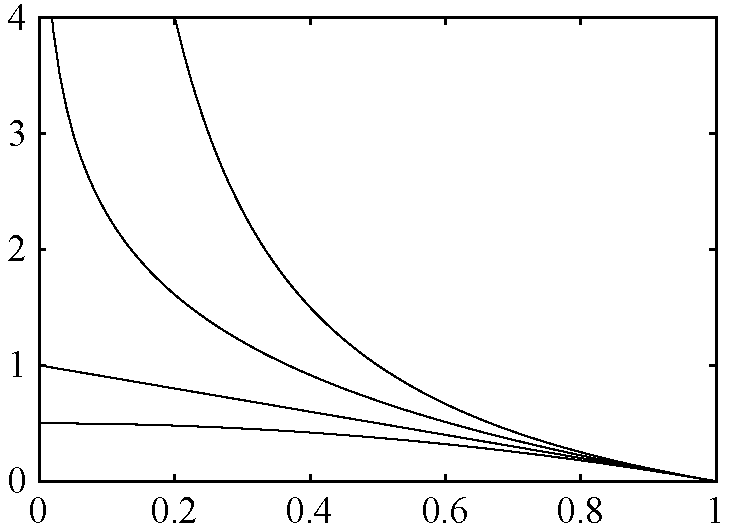
\includegraphics[height=50\unitlength]{surprise.pdf}}
\cell{60}{-4}{b}{$p$}
\cell{17}{25}{c}{$\ln_q(1/p)$}
\cell{49}{40}{c}{$q = 0$}
\cell{39}{30}{c}{$q = 1$}
\cell{35}{16}{c}{$q = 2$}
\cell{33}{6}{c}{$q = 3$}
\end{picture}
\caption{The functions $p \mapsto \ln_q(1/p)$ for several values of $q$.}
\lbl{fig:surprise-fns}
\end{figure}

\begin{examples}
\lbl{egs:q-ent} 
In these examples, we regard $\p = (p_1, \ldots, p_n) \in \Delta_n$ as the
relative abundance distribution of $n$ species making up a biological
community.  Sometimes $S_q(\p)$ has been advocated as a measure of
diversity (as in Patil and Taillie~\cite{PaTaDCM}, Keylock~\cite{Keyl}, and
Ricotta and Szeidl~\cite{RiSzTUA}), but this is problematic, as now
explained.  
% 
\begin{enumerate}
\item 
$S_0(\p) = |\supp(\p)| - 1$.  That is, the $0$-logarithmic entropy is one
  less than the number of species present.

\item
$S_1(\p) = H(\p)$.  The plague and oil company arguments of
  Examples~\ref{eg:plague} and~\ref{eg:oil} show why
$S_1$ should not be used as a diversity measure.  More generally, $S_q$
should not be used as a diversity measure either, for any value of $q$,
since it is not an effective number:
\[
S_q(\vc{u}_n) 
= 
\ln_q(n) 
\neq 
n.
\]
However, we will see in Section~\ref{sec:ren-hill} that $S_q$ can be
transformed into a well-behaved diversity measure, and that the result is
the Hill number of order $q$.

\item
\lbl{eg:q-ent-2}
The $2$-logarithmic entropy of $\p$ is
\[
S_2(\p)
=
1 - \sum_{i = 1}^n p_i^2
=
\sum_{i, j \csuch i \neq j} p_i p_j.
\]
This is the probability that two individuals chosen at random are of
different species.  In ecology, $S_2(\p)$ is associated with the names of
Edward H.~Simpson,%
%
\index{Simpson, Edward}
% 
who introduced $S_2(\p)$ as an index of diversity in 1949~\cite{SimpMD},
and Corrado Gini,%
%
\index{Gini, Corrado}
%
who used $S_2(\p)$ in a wide-ranging 1912 monograph on economics,
statistics and demography~\cite{Gini}.  It is such a natural quantity that
it has been used in many different fields; it also has the advantage that
it admits an unbiased estimator.  These points are discussed in the 1982
note of Good~\cite{GoodDCM},%
% 
\index{Good, Jack}
% 
who wrote that `any statistician of this century who wanted a measure of
homogeneity would have taken about two seconds to suggest $\sum p_i^2$\,'.

Despite all this, $S_2(\p)$ has the defect of not being an effective
number.  Again, Section~\ref{sec:ren-hill} describes the remedy.
\end{enumerate}
\end{examples}

\begin{remark}
\index{q-logarithmic entropy@$q$-logarithmic entropy!naming of}
\lbl{rmk:q-log-ent-name} 
%
The $q$-logarithmic entropies have been discovered and rediscovered
repeatedly.  They seem to have first appeared in a 1967 paper on
information and classification by Havrda%
%
\index{Havrda, Jan}
%
and Charv\'at~\cite{HaCh},%
%
\index{Charv\'at, Franti{\v{s}}ek}
%
in a form adapted to base~$2$ logarithms:
\[
\Si_q(\p)
=
\frac{1}{2^{1 - q} - 1} \biggl( \sum p_i^q - 1 \biggr)
\ntn{Sqi}
\]
The constant factor is chosen so that $\Si_q(\p)$ converges to the base~$2$
Shannon entropy $\Hi(\p)$ as $q \to 1$, and so that $\Si_q(\vc{u}_2) = 1$
for all $q$.

Further work on the entropies $\Si_q$ was carried out in 1968 by
Vajda~\cite{Vajd} (with reference to Havrda and Charv\'at).  They were
rediscovered in 1970 by Dar\'oczy~\cite{DaroGIF} (without reference to
Havrda and Charv\'at), and were the subject of Section~6.3 of the 1975
book~\cite{AcDa} by Acz\'el and Dar\'oczy (with reference to all of the
above).

The base~$e$ entropies $S_q$ themselves seem to have appeared first in
Section~3.2 of a 1982 paper~\cite{PaTaDCM} by Patil%
%
\index{Patil, Ganapata P.}
%  
and Taillie%
%
\index{Taillie, Charles} 
% 
(with reference to Acz\'el and Dar\'oczy but none of the others), where
$S_q$ was proposed as an index of biological diversity.

In physics, meanwhile, the $q$-logarithmic entropies appeared in a 1971
article of Lindhard and Nielsen~\cite{LiNi} (according to Csiszar
\cite{Csis}, Section~2.4).  They also made a brief appearance in a review
article on entropy in physics by Wehrl (\cite{Wehr}, p.~247).  Finally,
they were rediscovered again in a 1988 paper on statistical physics by
Tsallis~\cite{TsalPGB}%
%
\index{Tsallis, Constantino} 
% 
(with reference to none of the above).

Despite the twenty years of active life that the $q$-logarithmic entropies
had already enjoyed, it is after Tsallis that they are most commonly named.
The term `$q$-logarithmic entropy' is new, but has the benefits of being
descriptive and of not perpetuating a misattribution.
\end{remark}
\pagebreak

The chief advantage of the $q$-logarithmic entropies over the R\'enyi
entropies (introduced in Section~\ref{sec:ren-hill}) is that
they satisfy a simple chain rule:%
% 
\index{chain rule!q-logarithm@for $q$-logarithmic entropy}
% 
\begin{equation}
\lbl{eq:q-ent-chain}
S_q\bigl(\vc{w} \of (\p^1, \ldots, \p^n)\bigr)
=
S_q(\vc{w}) + \sum_{i \in \supp(\vc{w})} w_i^q S_q(\p^i)
\end{equation}
% 
($q \in \R$, $\vc{w} \in \Delta_n$, $\vc{p}^i \in \Delta_{k_i}$).  This is
easily checked directly.  Alternatively, one can imitate the proof of the
chain rule for Shannon entropy (Proposition~\ref{propn:ent-chain}), replacing
$\partial$ by $\partial_q \from x \mapsto x \ln_q(1/x)$ and showing that
\[
\partial_q(xy) = \partial_q(x)y + x^q \partial_q(y).
\]
We will also prove a more general chain rule as
Proposition~\ref{propn:q-ent-sim-ch}.

The special case $\p^1 = \cdots = \p^n = \p$ gives
% 
\begin{equation}
\lbl{eq:q-ent-mult}
S_q( \vc{w} \otimes \vc{p})
=
S_q(\vc{w}) + \Biggl( \sum_{i \in \supp(\vc{w})} w_i^q \Biggr) S_q(\p)  
\end{equation}
% 
($q \in \R$, $\vc{w} \in \Delta_n$, $\p \in \Delta_k$).  In particular, the
symmetry present in the case $q = 1$,
\[
H(\vc{w} \otimes \p) = H(\vc{w}) + H(\p),
\]
disappears when we deform away from $q = 1$. This is the key to the
characterization theorem that follows.  

Before we state it, let us record one other property: $S_q$ is
\demph{symmetric}\lbl{p:q-ent-sym},%
%
\index{symmetric!entropy}%
\index{symmetric!diversity measure} 
% 
meaning that
% 
\begin{equation}
\lbl{eq:q-ent-sym}
S_q(\p)
=
S_q(\p\sigma)
\end{equation}
% 
for all $q \in \R$, $\vc{p} \in \Delta_n$, and permutations $\sigma$ of
$\{1, \ldots, n\}$.

\begin{thm}
\lbl{thm:q-ent-char}
\index{q-logarithmic entropy@$q$-logarithmic entropy!characterization of}
% 
Let $1 \neq q \in \R$.  Let $(I \from \Delta_n \to \R)_{n \geq 1}$ be a
sequence of functions.  The following are equivalent:
% 
\begin{enumerate}
\item 
\lbl{part:q-ent-char-condns}
$I$ is symmetric and satisfies
\[
I( \vc{w} \otimes \vc{p})
=
I(\vc{w}) + \Biggl( \sum_{i \in \supp(\vc{w})} w_i^q \Biggr) I(\p)  
\]
for all $n, k \geq 1$, $\vc{w} \in \Delta_n$, and $\p \in \Delta_k$;

\item
\lbl{part:q-ent-char-form}
$I = cS_q$ for some $c \in \R$. 
\end{enumerate}
\end{thm}

This characterization of $q$-logarithmic entropy first appeared as
Theorem~III.1 of~\cite{SCRE}.  Notably, it needs no regularity conditions
whatsoever.  This is in contrast to the case $q = 1$ of Shannon entropy,
where some form of regularity is indispensable
(Remark~\ref{rmks:faddeev}\bref{rmk:faddeev-reg}).

\begin{proof}
By the observations just made, \bref{part:q-ent-char-form}
implies~\bref{part:q-ent-char-condns}.  Now
assume~\bref{part:q-ent-char-condns}.  By symmetry, $I(\vc{w} \otimes
\vc{p}) = I(\vc{p} \otimes \vc{w})$, so
\[
I(\vc{w}) + \Biggl( \sum_{i \in \supp(\vc{w})} w_i^q \Biggr) I(\vc{p})
=
I(\vc{p}) + \Biggl( \sum_{i \in \supp(\vc{p})} p_i^q \Biggr) I(\vc{w}),
\]
or equivalently,
\[
\Biggl( \sum_{i \in \supp(\vc{w})} w_i^q - 1 \Biggr) I(\vc{p})
=
\Biggl( \sum_{i \in \supp(\vc{p})} p_i^q - 1 \Biggr) I(\vc{w}),
\]
for all $\vc{w} \in \Delta_n$ and $\vc{p} \in \Delta_k$.  Take $\vc{w} =
\vc{u}_2$: then
\[
\bigl(2^{1 - q} - 1\bigr) I(\p)
=
\Biggl( \sum_{i \in \supp(\vc{p})} p_i^q - 1 \Biggr) I(\vc{u}_2)
\]
for all $\p \in \Delta_k$.  Since $q \neq 1$, we can define 
\[
c =
\frac{1 - q}{2^{1 - q} - 1}\,I(\vc{u}_2), 
\]
and then $I = cS_q$.
\end{proof}

\begin{remark}
\lbl{rmk:q-ent-char-hist} 
% 
There have been several characterization theorems for the $q$-logarithmic
entropies.  One similar to Theorem~\ref{thm:q-ent-char} was published
by Dar\'oczy%
%
\index{Dar\'oczy, Zolt\'an} 
% 
in 1970~\cite{DaroGIF}, and also appears as Theorem~6.3.9 of the book of
Acz\'el and Dar\'oczy~\cite{AcDa}.  In one sense it is stronger than
Theorem~\ref{thm:q-ent-char} (that is, has weaker hypotheses): where we
have assumed that $I \from \Delta_n \to \R$ is symmetric for all $n$,
Dar\'oczy assumed it only for $n = 3$.  On the other hand, Dar\'oczy's
theorem essentially assumed the full $q$-chain rule for $I(\vc{w} \of
(\p^1, \ldots, \p^n))$ (equation~\eqref{eq:q-ent-chain}), rather than just
the special case of $I(\vc{w} \otimes \p)$ that we used.

The word `essentially' here hides a historical wrinkle.  In
Remark~\ref{rmk:ent-chain-simp}, we noted that the chain rule for Shannon
entropy is equivalent to the special case
\[
H\bigl(pw_1, (1 - p)w_1, w_2, \ldots, w_n\bigr)
=
H(\vc{w}) + w_1 H(p, 1 - p),
\]
by a simple inductive argument.  Similarly, here, the $q$-chain rule of
equation~\eqref{eq:q-ent-chain} is equivalent to the special case
% 
\begin{equation}
\lbl{eq:q-ent-chain-simp}
S_q\bigl(pw_1, (1 - p)w_1, w_2, \ldots, w_n\bigr)
=
S_q(\vc{w}) + w_1^q S_q(p, 1 - p),
\end{equation}
% 
by the same simple inductive argument (given in Appendix~\ref{sec:chain}).
So, it is reasonable to regard~\eqref{eq:q-ent-chain}
and~\eqref{eq:q-ent-chain-simp} as equivalent.  But it was the special
case~\eqref{eq:q-ent-chain-simp}, not the general
case~\eqref{eq:q-ent-chain}, that was a hypothesis in Dar\'oczy's theorem.

The proof given by Dar\'oczy was entirely different, involving a
$q$-analogue of the `fundamental%
% 
\index{fundamental equation of information theory} 
% 
equation of information theory' (equation~\eqref{eq:feith}).

Other characterizations of $S_q$ have been proved, but using stronger
hypotheses than Theorem~\ref{thm:q-ent-char} to obtain the same conclusion
(such as the theorem in Section~2 of Suyari~\cite{Suya}, and Theorem~V.2
of Furuichi~\cite{Furu}).
\end{remark}

Just as ordinary entropy has a family of $q$-logarithmic deformations, so
too does relative entropy:

\begin{defn}
\lbl{defn:q-rel-ent}
Let $q \in \R$ and $\vc{p}, \vc{r} \in \Delta_n$.  The
\demph{$q$-logarithmic%
% 
\index{q-logarithmic relative entropy@$q$-logarithmic relative entropy}
% 
entropy of $\vc{p}$ relative to $\vc{r}$} is
\[
\srelent{q}{\vc{p}}{\vc{r}}
=
- \sum_{i \in \supp(\p)} p_i \ln_q \frac{r_i}{p_i}  
\in
[0, \infty].
\ntn{srelent}
\]
\end{defn}

Explicitly, $\srelent{1}{\vc{p}}{\vc{r}} = \relent{\vc{p}}{\vc{r}}$, and
for $q \neq 1$,
\[
\srelent{q}{\vc{p}}{\vc{r}}
=
\frac{1}{q - 1} \Biggl(
\sum_{i \in \supp(\p)} p_i^q r_i^{1 - q} - 1 
\Biggr).
\]
As for ordinary relative entropy $\relent{-}{-}$
(Section~\ref{sec:rel-defn}), we have
\[
\srelent{q}{\p}{\vc{r}} < \infty
\iff
(\vc{p}, \vc{r}) \in A_n.
\]

The definition of $q$-logarithmic relative entropy was given by
Rathie%
%
\index{Rathie, Pushpa N.} 
% 
and Kannappan%
%
\index{Kannappan, Palaniappan}
%   
in 1972~\cite{RaKa}.  (They used a version adapted to base~$2$ logarithms,
in the tradition of Havrda and Charv\'at described in
Remark~\ref{rmk:q-log-ent-name}.)  Their definition was taken up by Cressie
and Read in 1984 (\cite{CrRe}, Section~5), who used the base~$e$ version in
statistical work on goodness-of-fit tests.  It was rediscovered twice in
physics in 1998, by Shiino~\cite{Shii} and Tsallis~\cite{TsalGEB}
independently.

\begin{remark}
\lbl{rmk:q-rel-ent-param}
As in the definition of non-relative $q$-logarithmic entropy 
(Remark~\ref{rmk:q-ent-param}), there is a choice in how to generalize the
formula for ordinary relative entropy, given that $\ln_q(1/x) \neq
-\ln_q(x)$.  Again, making the other choice simply flips the
parametrization:
\[
\sum_{i \in \supp(\p)} p_i \ln_q \frac{p_i}{r_i}
=
\srelent{2 - q}{\vc{p}}{\vc{r}},
\]
by equation~\eqref{eq:q-log-reciprocal}.  The choice made in
Definition~\ref{defn:q-rel-ent} has the advantage that, as in the case $q =
1$, the relative entropy $\srelent{q}{\p}{\vc{u}_n}$ is a function of 
$S_q(\p)$ and $n$:
% 
\begin{align*}
\srelent{q}{\p}{\vc{u}_n}       &
=
n^{q - 1} \bigl( \ln_q(n) - S_q(\p) \bigr)      \\
&
=
n^{q - 1} \bigl( S_q(\vc{u}_n) - S_q(\p) \bigr),
\end{align*}
% 
as is easily checked.  
\end{remark}

Like its non-relative cousin, $q$-logarithmic relative entropy has an
extremely simple characterization.  It satisfies a chain rule
% 
\begin{multline*}
\srelEnt{q}{\vc{w} \of (\p^1, \ldots, \p^n)}%
{\twid{\vc{w}} \of (\twid{\p}^1, \ldots, \twid{\p}^n)}\\
=
\srelent{q}{\vc{w}}{\twid{\vc{w}}} + 
% \!\!
\sum_{i \in \supp(\vc{w})} w_i^q \twid{w}_i^{1 - q}
\srelEnt{q}{\p^i}{\twid{\p}^i}
\end{multline*}
% 
($\vc{w}, \twid{\vc{w}} \in \Delta_n$, $\p^i, \twid{\p}^i \in
\Delta_{k_i}$), which specializes to a multiplication rule
% 
\begin{equation}
\lbl{eq:q-rel-ent-mult}
\srelent{q}{\vc{w} \otimes \p}{\twid{\vc{w}} \otimes \twid{\p}}
=
\srelent{q}{\vc{w}}{\twid{\vc{w}}} + 
\Biggl( 
\sum_{i \in \supp(\vc{w})} w_i^q \twid{w}_i^{1 - q}
\Biggr) 
\srelent{q}{\p}{\twid{\p}}
\end{equation}
% 
($\vc{w}, \twid{\vc{w}} \in \Delta_n$, $\p, \twid{\p} \in \Delta_k$).
Moreover, $\srelent{q}{-}{-}$ is permutation-invariant in the same
sense as in the case $q = 1$ (Section~\ref{sec:rel-defn}).
Equation~\eqref{eq:q-rel-ent-mult} and permutation-invariance characterize
$\srelent{q}{-}{-}$ uniquely up to a constant factor:

\begin{thm}
\lbl{thm:q-rel-ent-char}
\index{q-logarithmic relative entropy@$q$-logarithmic relative entropy!characterization of}
% 
Let $1 \neq q \in \R$.  Let $\bigl(\melent{-}{-} \from A_n \to \R\bigr)_{n
  \geq 1}$ be a sequence of functions.  The following are equivalent:
% 
\begin{enumerate}
\item 
\lbl{part:q-rel-ent-char-condns}
$\melent{-}{-}$ is permutation-invariant and satisfies the multiplication
rule~\eqref{eq:q-rel-ent-mult} (with $I$ in place of $S_q$);

\item
\lbl{part:q-rel-ent-char-form}
$\melent{-}{-} = c\srelent{q}{-}{-}$ for some $c \in \R$.
\end{enumerate}
\end{thm}

This result first appeared as Theorem~IV.1 of~\cite{SCRE}.  Compared with
the characterization theorem for ordinary relative entropy
(Theorem~\ref{thm:rel-char}), it needs neither a regularity condition nor
the vanishing axiom.

\begin{proof}
The proof is very similar to that of Theorem~\ref{thm:q-ent-char}.
By the observations just made, \bref{part:q-rel-ent-char-form}
implies~\bref{part:q-rel-ent-char-condns}.  Now
assume~\bref{part:q-rel-ent-char-condns}.  By permutation-invariance,
\[
\melent{\vc{p} \otimes \vc{r}}{\twid{\vc{p}} \otimes \twid{\vc{r}}}
=
\melent{\vc{r} \otimes \vc{p}}{\twid{\vc{r}} \otimes \twid{\vc{p}}}
\]
for all $(\p, \twid{\p}) \in A_n$ and $(\vc{r}, \twid{\vc{r}})
\in A_k$.  So by the multiplication rule,
\[
\melent{\vc{p}}{\twid{\vc{p}}}
+ 
\biggl( \sum p_i^q \twid{p}_i^{1 - q} \biggr)
\melent{\vc{r}}{\twid{\vc{r}}}
=
\melent{\vc{r}}{\twid{\vc{r}}}
+ 
\biggl( \sum r_i^q \twid{r}_i^{1 - q} \biggr)
\melent{\p}{\twid{\p}},
\]
or equivalently,
\[
\biggl( \sum r_i^q \twid{r}_i^{1 - q} - 1 \biggr) 
\melent{\vc{p}}{\twid{\vc{p}}}
=
\biggl( \sum p_i^q \twid{p}_i^{1 - q} - 1 \biggr) 
\melent{\vc{r}}{\twid{\vc{r}}}.
\]
Take $\vc{r} = (1, 0)$ and $\twid{\vc{r}} = \vc{u}_2$: then
\[
(2^{q - 1} - 1) \melent{\vc{p}}{\twid{\vc{p}}}
=
\melent{(1, 0)}{\vc{u}_2} 
\biggl( \sum p_i^q \twid{p}_i^{1 - q} - 1 \biggr)
\]
for all $(\p, \twid{\p}) \in A_n$.  Since $q \neq 1$, we can put 
\[
c 
=
\frac{(q - 1)\melent{(1, 0)}{\vc{u}_2}}{2^{q - 1} - 1},
\]
and then $\melent{-}{-} = c \srelent{q}{-}{-}$.
\end{proof}

\begin{remark}
Other characterization theorems for $q$-logarithmic relative entropy have
been proved.  For example, Furuichi (\cite{Furu}, Section~IV) obtained the
same conclusion, but also assumed continuity and the full chain rule (or
more precisely, an equivalent special case, as in
Remark~\ref{rmk:q-ent-char-hist}) instead of just the multiplication
rule~\eqref{eq:q-rel-ent-mult}.
\end{remark}


\section{Power means}
\lbl{sec:pwr-mns}


We pause in our account of deformations of Shannon entropy to collect some
basic facts about power means (also called generalized means).  The reason
for doing this now is that the language and theory of power means make
possible a considerable streamlining of later material on R\'enyi entropies
and diversity measures.

The reader not interested in means for their own sake may wish to read 
Definition~\ref{defn:pwr-mn} and then jump ahead
to Section~\ref{sec:ren-hill}, referring back here only as necessary.  

This
section is essentially a list of properties satisfied by the power means,
together with the terminology for those properties.  A summary of the
terminology can also be found in Appendix~\ref{app:condns}.
% 
Means are a classical topic of analysis, and almost everything in this
section can be found in Chapter~II of Hardy, Littlewood and P\'olya's
book~\cite{HLP}.

In what follows, $n$ denotes a positive integer.

\begin{defn}
\lbl{defn:pwr-mn}
Let $t \in [-\infty, \infty]$, $\p \in \Delta_n$, and $\vc{x} \in [0,
\infty)^n$.  The \demph{power%
%
\index{power mean} 
% 
mean of order%
%
\index{order!power mean@of power mean}
% 
$t$ of $\vc{x}$, weighted by $\p$}, is defined for $0 < t < \infty$ by
% 
\begin{equation}
\lbl{eq:defn-pwr-mn}
M_t(\p, \vc{x})
=
\Biggl( \sum_{i \in \supp(\p)} p_i x_i^t \Biggr)^{1/t},
\end{equation}
% 
for $-\infty < t < 0$ by
% 
\begin{equation}
\lbl{eq:defn-pwr-mn-neg}
M_t(\p, \vc{x})
=
\begin{cases}
\displaystyle
\Biggl( \sum_{i \in \supp(\p)} p_i x_i^t \Biggr)^{1/t}  &
\text{if } x_i > 0 \text{ for all } i \in \supp(\p),    \\
\displaystyle
0       &
\text{otherwise},
\end{cases}
\end{equation}
% 
and for the remaining values of $t$ by 
% 
\begin{align*}
M_{-\infty}(\p, \vc{x}) &
=
\min_{i \in \supp(\p)} x_i,     \\
M_0(\p, \vc{x}) &
=
\prod_{i \in \supp(\p)} x_i^{p_i},      \\
M_\infty(\p, \vc{x})    &
=
\max_{i \in \supp(\p)} x_i.
\end{align*}
% 
\end{defn}

The various exceptional cases in this definition are justified by
continuity, as detailed after the following examples.

\begin{examples}
\begin{enumerate}
\item 
The mean of order $1$ is the arithmetic\index{mean!arithmetic} mean $\sum
p_i x_i$ of $\vc{x}$ weighted by $\p$.

\item
The mean of order $0$ is the geometric\index{mean!geometric} mean of
$\vc{x}$ weighted by $\p$.

\item
The mean of order $-1$ is the harmonic\index{mean!harmonic} mean
\[
\frac{1}{\frac{p_1}{x_1} + \cdots + \frac{p_n}{x_n}}
\]
of $\vc{x}$ weighted by $\p$.
\end{enumerate}
\end{examples}

\begin{example}
Taking $\p = \vc{u}_n$ gives the \demph{unweighted}%
%
\index{power mean!unweighted}%
\index{mean!unweighted} 
%
(or uniformly weighted) power means $M_t(\vc{u}_n, \vc{x})$.
\end{example}

\begin{example}
For each $t \in [-\infty, \infty]$, the power mean $M_t$ has at least the
basic properties of an average:
\[
M_t\bigl(\p, (x, \ldots, x)\bigr) = x
\]
for all $\p \in \Delta_n$ and $x \in [0, \infty)$, and
\[
\min_{i \in \supp(\p)} x_i
\leq
M_t(\p, \vc{x})
\leq
\max_{i \in \supp(\p)} x_i
\]
for all $\p \in \Delta_n$ and $\vc{x} \in [0, \infty)^n$.  The rest of this
section is devoted to investigating the properties of power means in
greater depth.
\end{example}

We now prove three statements on the continuity of power means $M_t(\p,
\vc{x})$.  The first is on continuity in $\vc{x}$.

\begin{lemma}
\lbl{lemma:pwr-mns-cts-x}
\index{power mean!continuity of}
% 
Let $t \in [-\infty, \infty]$ and $\p \in \Delta_n$.  Then the function
\[
M_t(\p, -) \from [0, \infty)^n \to [0, \infty)
\]
is continuous.
\end{lemma}

\begin{proof}
Let $\vc{x} \in [0, \infty)^n$.  From Definition~\ref{defn:pwr-mn}, it is
immediate that $M_t(\p, \vc{x})$ is continuous at $\vc{x}$ except perhaps
in the case where $t \in (-\infty, 0)$ and $x_i = 0$ for some $i \in
\supp(\p)$.  So, let $t \in (-\infty, 0)$ and suppose that, say, $x_1 =
0$ with $1 \in \supp(\p)$.  It suffices to show that $M_t(\p, \vc{y}) \to
0$ as $\vc{y} \to \vc{x}$ with $y_i > 0$ for all $i \in \supp(\p)$.  And
indeed, for such $\vc{y}$,
% 
\begin{align*}
\bigl| M_t(\p, \vc{y}) \bigr|   &
=
\Biggl( \sum_{i \in \supp(\p)} p_i y_i^t \Biggr)^{1/t}  \\
&
\leq
\bigl( p_1 y_1^t \bigr)^{1/t}   \\
&
=
p_1^{1/t} y_1   \\
&
\to 
p_1^{1/t} x_1
=
0
\end{align*}
% 
as $\vc{y} \to \vc{x}$, as required.
\end{proof}

The continuity properties of $M_t(\p, \vc{x})$ in $\p$ are more delicate.
Indeed, the power means of order $\leq 0$ are \emph{not} continuous in
$\p$: for when $t \leq 0$,
\[
M_t\bigl((\epsln, 1 - \epsln), (0, 1)\bigr) = 0
\]
for all $\epsln \in (0, 1]$, whereas
\[
M_t\bigl((0, 1), (0, 1)\bigr) = 1.
\]
Discontinuities do not only arise from zero values of $x_i$.  For
instance, $M_{-\infty}(\p, (1, 2))$ is not continuous in $\p$, since
\[
M_{-\infty}\bigl((\epsln, 1 - \epsln), (1, 2)\bigr) = 1,
\quad
M_{-\infty}\bigl((0, 1), (1, 2)\bigr) = 2
\]
for all $\epsln \in (0, 1]$.  There is a similar counterexample for
$M_\infty$.  But we do have the following.

\begin{lemma}
\lbl{lemma:pwr-mns-cts-px}
\index{power mean!continuity of}
% 
\begin{enumerate}
\item 
\lbl{part:pwr-mns-cts-px-1}
For all $t \in [-\infty, \infty]$, the function
\[
M_t(-, -) \from \Delta_n^\circ \times [0, \infty)^n \to [0, \infty)
\]
is continuous.

\item 
\lbl{part:pwr-mns-cts-px-3}
For all $t \in (-\infty, \infty)$, the function
\[
M_t(-, -) \from \Delta_n \times (0, \infty)^n \to (0, \infty)
\]
is continuous.

\item 
\lbl{part:pwr-mns-cts-px-2}
For all $t \in (0, \infty)$, the function
\[
M_t(-, -) \from \Delta_n \times [0, \infty)^n \to [0, \infty)
\]
is continuous.
\end{enumerate}
\end{lemma}

\begin{proof}
Part~\bref{part:pwr-mns-cts-px-1} is immediate from the definition.  For
parts~\bref{part:pwr-mns-cts-px-3} and~\bref{part:pwr-mns-cts-px-2}, just
note that in the cases at hand, the formulas for $M_t$ are unchanged if $i$
is allowed to range over all of $\{1, \ldots, n\}$ instead of only
$\supp(\p)$.
\end{proof}

Our third and final continuity lemma states that power means are continuous
in their order.

\begin{lemma}
\lbl{lemma:pwr-mns-cts-t}
\index{power mean!continuity of}
% 
Let $\p \in \Delta_n$ and $\vc{x} \in [0, \infty)^n$.  Then $M_t(\p,
  \vc{x})$ is continuous in $t \in [-\infty, \infty]$.
\end{lemma}

\begin{proof}
This is clear except perhaps at $t = 0$ and $t = \pm \infty$.  

For continuity at $t = 0$, first suppose that $x_i > 0$ for all $i \in
\supp(\p)$.  When $t$ is finite and nonzero, 
% 
\begin{equation}
\lbl{eq:log-mn-hop}
% \[
\log M_t(\p, \vc{x})
=
\frac{\log \bigl(\sum_{i \in \supp(\p)} p_i x_i^t\bigr)}{t}.
% \]
\end{equation}
% 
As $t \to 0$, 
\[
\log \Biggl(\sum_{i \in \supp(\p)} p_i x_i^t\Biggr)
\to
\log \Biggl(\sum_{i \in \supp(\p)} p_i\Biggr)
=
0,
\]
so we can apply l'H\^opital's rule to equation~\eqref{eq:log-mn-hop}, giving
% 
\begin{align*}
\lim_{t \to 0} \log M_t(\p, \vc{x})     &
% =
% \lim_{t \to 0} 
% \frac{\tfrac{d}{dt} \log \sum p_i x_i^t}{\tfrac{d}{dt} t}       \\
% &
=
\lim_{t \to 0} 
\frac{\sum p_i x_i^t \log x_i}{\sum p_i x_i^t}  \\
&
=
\sum p_i \log x_i       \\
&
=
\log M_0(\vc{p}, \vc{x}),
\end{align*}
% 
where all sums are over $i \in \supp(\p)$.  Hence the map $t \mapsto M_t(\p,
\vc{x})$ is continuous at $t = 0$.   

Now suppose that $x_i = 0$ for some $i \in \supp(\p)$.  By definition,
$M_t(\p, \vc{x}) = 0$ for all $t \leq 0$, so it suffices to show that
$M_t(\p, \vc{x}) \to 0$ as $t \to {0+}$.  For $t \in (0, \infty)$,
\[
0 
\leq 
M_t(\p, \vc{x}) 
=
\Biggl( \sum_{i \in \supp(\p)} p_i x_i^t \Biggr)^{1/t}
\leq 
M_\infty(\p, \vc{x}) \cdot
\Biggl(\sum_{i \in \supp(\p) \cap \supp(\vc{x})} p_i\Biggr)^{1/t}.
\]
But $\sum_{i \in \supp(\p) \cap \supp(\vc{x})} p_i < 1$, so our upper
  bound on $M_t(\p, \vc{x})$ converges to $0$ as $t \to {0+}$.  Hence also
  $M_t(\p, \vc{x}) \to 0$ as $t \to {0+}$, as required.

For continuity at $t = \infty$, suppose without loss of generality that
$\max_{i \in \supp(\p)} x_i$ is achieved at $i = 1$.  Then for $t \in (0,
\infty)$, 
\[
M_t(\p, \vc{x}) 
\leq
\Biggl( \sum_{i \in \supp(\p)} p_i x_1^t \Biggr)^{1/t}
=
x_1.
\]
On the other hand,
\[
M_t(\p, \vc{x}) 
\geq
\bigl( p_1 x_1^t \bigr)^{1/t}
=
p_1^{1/t} x_1
\to
x_1
\]
as $t \to \infty$.  Hence 
\[
M_t(\p, \vc{x}) \to x_1 = M_\infty(\p, \vc{x})
\]
as $t \to \infty$, as required.  The proof for $M_{-\infty}$ is similar.
\end{proof}

We now come to the celebrated inequality of the arithmetic and geometric
means:
\[
\frac{1}{n} \sum_{i = 1}^n x_i
\geq
\Biggl( \prod_{i = 1}^n x_i \Biggr)^{1/n}
\]
for all $x_1, \ldots, x_n \geq 0$.  This is a very special case of the
following classical and fundamental result (Theorem~9 of Hardy, Littlewood
and P\'olya~\cite{HLP}, for instance).  Recall from
Remark~\ref{rmk:defn-inc} that we use the word `increasing' in the
non-strict sense.

\begin{thm}
\lbl{thm:mns-inc-ord}
\index{power mean!decreasing in order@is decreasing in order}
% 
Let $\p \in \Delta_n$ and $\vc{x} \in [0, \infty)^n$, with $x_i > 0$ for
  all $i \in \supp(\p)$.  Then the function
\[
\begin{array}{ccc}
[-\infty, \infty]       &\to            &[0, \infty)   \\
t                       &\mapsto        &M_t(\p, \vc{x})
\end{array}
\]
is increasing.  It is constant if $x_i = x_j$ for all $i, j \in \supp(\p)$,
and strictly increasing otherwise.
\end{thm}

\begin{proof}
If the coordinates $x_i$ of $\vc{x}$ have the same value $x$ for all $i \in
\supp(\p)$, then evidently $M_t(\p, \vc{x}) = x$ for all $t \in [-\infty,
  \infty]$.  Supposing otherwise, we have to prove that $M_t(\p, \vc{x})$
is strictly increasing in $t \in [-\infty, \infty]$.  We will prove that
$\tfrac{d}{dt} \log M_t(\p, \vc{x}) > 0$ for all $t \in (-\infty, 0) \cup
(0, \infty)$.  Since $M_t(\p, \vc{x})$ is continuous in $t \in [-\infty,
  \infty]$ (Lemma~\ref{lemma:pwr-mns-cts-t}), this suffices.  For real $t
\neq 0$, 
% 
\begin{align}
\frac{d}{dt} \log M_t(\p, \vc{x})      &
=
\frac{d}{dt} \Biggl( \frac{\log \sum p_i x_i^t}{t} \Biggr)      
\nonumber       \\
&
=
\frac{t \bigl(\sum p_i x_i^t \log x_i\bigr)/
\bigl(\sum p_i x_i^t\bigr) - \log \sum p_i x_i^t}%
{t^2}   
\nonumber       \\
&
=
\frac{\sum p_i x_i^t \log x_i^t 
- \bigl(\sum p_i x_i^t\bigr) \log \sum p_i x_i^t}%
{t^2 \sum p_i x_i^t}    
\nonumber       \\
&
=
\frac{- \sum p_i \partial(x_i^t) + \partial \bigl(\sum p_i x_i^t\bigr)}%
{t^2 \sum p_i x_i^t},
\lbl{eq:log-M-conc}
\end{align}
% 
where all sums are over $i \in \supp(\p)$ and $\partial(x) = -x\log x$ (as
in equation~\eqref{eq:defn-par}).  But $\partial''(x) = -1/x < 0$ for all
$x > 0$, so $\partial$ is strictly concave.  Hence by
equation~\eqref{eq:log-M-conc},
\[
\tfrac{d}{dt} \log M_t(\p, \vc{x}) \geq 0,
\]
with equality if and only if $x_i^t = x_j^t$ for all $i, j \in \supp(\p)$.
But $t \neq 0$, so equality only holds if $x_i = x_j$ for all $i, j \in
\supp(\p)$, contrary to our earlier assumption.  Hence the inequality is
strict, as required.
\end{proof}

There is a simple duality%
% 
\index{power mean!duality for}%
\index{duality for power means}
% 
law for power means: 
% 
\begin{equation}
\lbl{eq:mn-duality}
M_{-t}(\p, \vc{x}) 
=
\frac{1}{M_t(\p, 1/\vc{x})}
\end{equation}
% 
for all $t \in [-\infty, \infty]$, $\p \in \Delta_n$, and $\vc{x} \in (0,
\infty)^n$.  Here $1/\vc{x}$ denotes the vector $(1/x_1, \ldots,
1/x_n)$.  For instance, in the case $t = 1$, the harmonic mean is the
reciprocal of the arithmetic means of $1/x_1, \ldots, 1/x_n$.

\begin{remark}
\lbl{rmk:vec-op-conv}
Often in this text, we will want to perform coordinatewise algebraic
operations on vectors.\index{vector!operations}  For instance, given
$\vc{x}, \vc{y} \in \R^n$, we will use not only the (coordinatewise) sum
and difference $\vc{x} + \vc{y}$ and $\vc{x} - \vc{y}$, but also the
coordinatewise product and quotient
\[
\vc{x}\vc{y} = (x_1 y_1, \ldots, x_n y_n),
\qquad
\vc{x}/\vc{y} = (x_1/y_1, \ldots, x_n/y_n)
\ntn{vecops}
\]
(with the usual caveats regarding $y_i = 0$ in the latter case).  This is
just the standard notation for the product and quotient of real-valued
functions on a set $S$, applied to $S = \{1, \ldots, n\}$.
\end{remark}

We now run through some basic properties satisfied by the power means 
\[
\bigl( 
M_t \from \Delta_n \times [0, \infty)^n \to [0, \infty) 
\bigr)_{n \geq 1}
\]
of every order $t \in [-\infty, \infty]$.  For later purposes, it is useful
to set up the terminology in the generality of a sequence of functions
\[
\bigl( 
M \from \Delta_n \times I^n \to I
\bigr)_{n \geq 1},
\]
where $I$ is an arbitrary real interval.  The most important cases are $I =
[0, \infty)$ and $I = (0, \infty)$.

\begin{defn}
\lbl{defn:pwr-mn-elem}
Let $I$ be a real interval and let $(M \from \Delta_n \times I^n \to I)_{n
  \geq 1}$ be a sequence of functions.
% 
\begin{enumerate}
\item 
\lbl{part:pme-sym}
$M$ is \demph{symmetric}%
% 
\index{symmetric!weighted mean}
% 
if $M(\p, \vc{x}) = M(\p\sigma, \vc{x}\sigma)$ for
  all $n \geq 1$, $\p \in \Delta_n$, $\vc{x} \in I^n$, and permutations
  $\sigma$ of $\{1, \ldots, n\}$, where $\p\sigma$ and $\vc{x}\sigma$ are
  defined as in equation~\eqref{eq:p-perm}.

\item
\lbl{part:pme-abs}
$M$ is \demph{absence-invariant}%
%
\index{absence-invariance!mean@of mean}
%
if whenever $\p \in \Delta_n$, $\vc{x} \in I^n$ and $1 \leq i \leq n$ with
$p_i = 0$, then
\[
M(\p, \vc{x})
=
M\bigl(
(p_1, \ldots, p_{i - 1}, p_{i + 1}, \ldots, p_n),
(x_1, \ldots, x_{i - 1}, x_{i + 1}, \ldots, x_n)
\bigr).
\]

\item
$M$ has the \demph{repetition}%
% 
\index{repetition}
% 
property if
whenever $\p \in \Delta_n$, $\vc{x} \in I^n$ and $1 \leq i < n$ with $x_i
= x_{i + 1}$, then
% 
\begin{multline*}
M(\p, \vc{x}) 
\\
=
M\bigl(
(p_1, \ldots, p_{i - 1}, p_i + p_{i + 1}, p_{i + 2}, \ldots, p_n),
(x_1, \ldots, x_{i - 1}, x_i, x_{i + 2}, \ldots, x_n)
\bigr).
\end{multline*}
\end{enumerate}
\end{defn}

Absence-invariance states that $M$ behaves logically with respect to
elements $x_i$ that are absent (have zero weight): such elements might as
well be ignored.

\begin{lemma}
\lbl{lemma:pwr-mns-elem}
\index{power mean!symmetry of}
\index{power mean!absence-invariance of}
\index{power mean!repetition for} 
% 
Let $t \in [-\infty, \infty]$.  Then $M_t$ has the symmetry,
absence-invariance and repetition properties.
\end{lemma}

A direct proof of this lemma is, of course, elementary, but it is
enlightening to derive all three properties from a single general law, as
follows.  Let
\[
f \from \{1, \ldots, m\} \to \{1, \ldots, n\}
\]
be a map of finite sets.  Any distribution $\p \in \Delta_m$ gives rise to
a pushforward distribution $f \p \in \Delta_n$
(Definition~\ref{defn:pfwd}).  On the other hand, any vector $\vc{x} \in
[0, \infty)^n$ can be pulled back along $f$ to give a vector $\vc{x}f \in
  [0, \infty)^m$, where
\[
(\vc{x}f)_i = x_{f(i)}
\ntn{xf}
\]
($i \in \{1, \ldots, m\}$).  

\begin{defn}
\lbl{defn:mn-nat}
Let $I$ be a real interval.  A sequence of functions $\bigl( M \from
\Delta_n \times I^n \to I \bigr)_{n \geq 1}$ is
\demph{natural}%
%
\index{naturality!weighted mean@of weighted mean} 
% 
if  
\[
M(f\vc{p}, \vc{x}) = M(\vc{p}, \vc{x}f)
\]
for all $m, n \geq 1$, $\vc{p} \in \Delta_m$, $\vc{x} \in I^n$, and maps of
sets 
\[
f \from \{1, \ldots, m\} \to \{1, \ldots, n\}.
\]
\end{defn}

\begin{remark}
If we write $x_j$ as $\phi(j)$, so that $\phi$ is a function $\{1, \ldots,
n\} \to [0, \infty)$, then $\vc{x}f = \phi \of f$.  If we also write
$M(\p, -)$ as $\int - \dee\p$ then naturality states that
\[
\int \phi \dee(f \p) = \int (\phi \of f) \dee\p,
\]
the standard formula for integration under a change%
% 
\index{change of variable}
% 
of variable.  However, this notation is misleading: unlike an ordinary
integral, $M(\p, \vc{x})$ need not be linear in $\vc{x}$ (and is not when
$M = M_t$ for $t \neq 1$).
\end{remark}

\begin{lemma}[Naturality]
\lbl{lemma:pwr-mns-nat}
\index{power mean!naturality of}
% 
For each $t \in [-\infty, \infty]$, the power mean $M_t$ on $[0, \infty)$
  is natural.
\end{lemma}

\begin{proof}
Take $\p$, $\vc{x}$, and $f$ as in Definition~\ref{defn:mn-nat}.  We have to
show that $M_t(f\p, \vc{x}) = M_t(\p, \vc{x}f)$.  First suppose that $t
\neq 0, \pm\infty$ and that $x_j > 0$ for all $j \in \{1, \ldots, n\}$.
Then
% 
\begin{align*}
M_t(f\p, \vc{x})     &
=
\Biggl( \sum_{j \in \supp(f\p)} (f \p)_j x_j^t \Biggr)^{1/t}    \\
&
=
\Biggl( 
\sum_{\,j \in \supp(f\p)\ } \sum_{i \in f^{-1}(j)} p_i x_j^t 
\Biggr)^{1/t}   \\
&
=
\Biggl( \sum_{\,i \in \supp(\p)\,} p_i x_{f(i)}^t \Biggr)^{1/t}     \\
&
=
M_t(\p, \vc{x}f),
\end{align*}
% 
as required.  The case where $x_j = 0$ for some values of $j$ follows by
continuity of $M_t(\p, \vc{x})$ in $\vc{x}$
(Lemma~\ref{lemma:pwr-mns-cts-x}), and the result for $t = 0$ and $t =
\pm\infty$ follows by continuity of $M_t$ in $t$
(Lemma~\ref{lemma:pwr-mns-cts-t}).  
\end{proof}

\begin{pfof}{Lemma~\ref{lemma:pwr-mns-elem}}\lbl{p:lpme-pf}
We use the naturality of the power means
for all three parts.  Write $\lwr{n} = \{1, \ldots, n\}$.  Symmetry follows
by taking $f$ to be a bijection $\lwr{n} \to \lwr{n}$.
Absence-invariance follows by taking $f$ to be the order-preserving
injection $\lwr{n - 1} \to \lwr{n}$ that omits $i$ from its image.  The
repetition property follows by taking $f$ to be the order-preserving
surjection $\lwr{n} \to \lwr{n - 1}$ that identifies $i$ with $i + 1$.
\end{pfof}

\begin{remark}
\lbl{rmk:defined-even-if-not}
The absence-invariance of the power means implies that $M_t(\p, \vc{x})$
is unaffected by the value of $x_i$ for coordinates $i$ such that $p_i =
0$.  Indeed, writing $\supp(\p) = \{i_1, \ldots, i_k\}$ with $i_1 < \cdots
< i_k$, we have
\[
M_t(\p, \vc{x})
=
M_t\bigl( (p_{i_1}, \ldots, p_{i_k}), (x_{i_1}, \ldots, x_{i_k})\bigr)
\]
for all $\vc{x}$, by absence-invariance and induction.  Hence
\[
M_t(\p, \vc{x}) = M_t(\p, \vc{y})
\]
whenever $\vc{x}, \vc{y} \in [0, \infty)^n$ with $x_i = y_i$ for all $i \in
\supp(\p)$.

Because of this, the expression $M_t(\p, \vc{x})$ has a clear meaning even
if $x_i$ is \emph{undefined} for some or all $i \not\in \supp(\p)$.  (We
can arbitrarily put $x_i = 0$ or $x_i = 17$ for all such $i$;
it makes no difference.)  For example, the expression
\[
M_t(\p, 1/\p)
\]
has a clear meaning for all $\p \in \Delta_n$, even if $p_i = 0$ for some
$i$; writing $\supp(\p) = \{i_1, \ldots, i_k\}$ as above, it is understood
to mean
\[
M_t\bigl( (p_{i_1}, \ldots, p_{i_k}), (1/p_{i_1}, \ldots, 1/p_{i_k})\bigr).
\]

\femph{We adopt the convention%
% 
\index{power mean!undefined arguments@with undefined arguments}%
\index{undefined arguments}
% 
throughout this text} that power means
$M_t(\p, \vc{x})$ are valid expressions even if $x_i$ is undefined for some
$i \not\in \supp(\p)$, and are to be interpreted as just described.  This
convention is strictly analogous to the standard interpretation of integral
notation $\int f \dee\mu$, for a function $f$ and a measure $\mu$: the
integral is unaffected by the value of $f$ off the support of $\mu$, and
has an unambiguous meaning even if $f$ is undefined there.
\end{remark}

A minimal requirement on anything called a mean is that the mean of
several copies of $x$ should be $x$:

\begin{defn}
\lbl{defn:w-cons}
Let $I$ be a real interval.  A sequence of functions $(M \from \Delta_n
\times I^n \to I)_{n \geq 1}$ is \demph{consistent}%
%
\index{consistent!weighted mean} 
% 
if
\[
M\bigl(\p, (x, \ldots, x)\bigr) = x
\]
for all $n \geq 1$, $\vc{p} \in \Delta_n$, and $x \in I$.
\end{defn}

\begin{lemma}
\lbl{lemma:pwr-mns-con}
\index{power mean!consistency of}
% 
For each $t \in [-\infty, \infty]$, the power mean $M_t$ 
% on $[0, \infty)$ 
is consistent.
\end{lemma}

\begin{proof}
Trivial.
\end{proof}

For $\vc{x}, \vc{y} \in \R^n$, write $\vc{x} \leq\ntn{leq} \vc{y}$ if $x_i
\leq y_i$ for all $i \in \{1, \ldots, n\}$.

\begin{defn}
\lbl{defn:w-isi}
Let $I$ be a real interval and let $( M \from \Delta_n \times I^n \to I)_{n
  \geq 1}$ be a sequence of functions.
% 
\begin{enumerate}
\item
$M$ is \demph{increasing}%
% 
\index{increasing!weighted mean}%
\index{mean!increasing}
% 
if 
\[
\vc{x} \leq \vc{y}
\implies
M(\p, \vc{x}) \leq M(\p, \vc{y})
\]
for all $n \geq 1$, $\vc{p} \in \Delta_n$, and $\vc{x}, \vc{y} \in I^n$.

\item
$M$ is \demph{strictly increasing}%
% 
\index{strictly increasing!weighted mean}%
\index{mean!strictly increasing}%
\index{increasing!strictly}
% 
if 
\[
\bigl( \vc{x} \leq \vc{y} \text{ and } 
x_i < y_i \text{ for some } i \in \supp(\p) \bigr)
\implies
M(\p, \vc{x}) < M(\p, \vc{y})
\]
for all $n \geq 1$, $\vc{p} \in \Delta_n$, and $\vc{x}, \vc{y} \in I^n$. 
\end{enumerate}
\end{defn}

Whether the power mean $M_t$ is \emph{strictly} increasing depends on both
the order $t$ and whether the domain of definition is taken to be $[0,
  \infty)$ or $(0, \infty)$, as follows.

\begin{lemma}
\lbl{lemma:pwr-mns-inc}
% Let $t \in [-\infty, \infty]$.
\begin{enumerate}
\item
For all $t \in [-\infty, \infty]$, the power mean $M_t$ on $[0, \infty)$ is
  increasing. 

\item
For all $t \in (-\infty, \infty)$, the power mean $M_t$ on $(0, \infty)$ is
strictly increasing. 

\item
For all $t \in (0, \infty)$, the power mean $M_t$ on $[0, \infty)$ is strictly
  increasing.
\end{enumerate}
\end{lemma}

\begin{proof}
Elementary.
\end{proof}

\begin{remark}
\lbl{rmk:pwr-mns-not-si}
The careful statement of Lemma~\ref{lemma:pwr-mns-inc} is necessary because
of various limiting counterexamples.  The means $M_{\pm\infty}$ are not
strictly increasing on $(0, \infty)$, since, for instance,
\[
M_\infty\bigl(\vc{u}_2, (1, 3)\bigr) 
=
3 
= 
M_\infty\bigl(\vc{u}_2, (2, 3)\bigr).
\]
When $t \in [-\infty, 0]$, the mean $M_t$ is not strictly increasing on
$[0, \infty)$; for example,
\[
M_t\bigl( \vc{u}_2, (0, 1)\bigr)
=
0
=
M_t\bigl( \vc{u}_2, (0, 2)\bigr).
\]
% by definition of $M_t$.
\end{remark}

\begin{defn}
\lbl{defn:w-mn-hgs}
Let $I$ be a real interval closed under multiplication.  A sequence of
functions $(M \from \Delta_n \times I^n \to I)_{n \geq 1}$ is
\demph{homogeneous}%
%
\index{homogeneous!weighted mean} 
% 
if 
\[
M(\p, c\vc{x}) = cM(\p, \vc{x})
\]
for all $n \geq 1$, $\p \in \Delta_n$, $c \in I$, and $\vc{x} \in I^n$.
\end{defn}

The hypothesis on $I$ guarantees that $M(\p, c\vc{x})$ is defined.
% The only cases we will consider are $I = [0, \infty)$ and $I =
% (0, \infty)$.  

\begin{lemma}
\lbl{lemma:pwr-mns-hgs}
\index{power mean!homogeneity of}
% 
For each $t \in [-\infty, \infty]$, the power mean $M_t$ on $[0, \infty)$
is homogeneous.  
\end{lemma}

\begin{proof}
Elementary.
\end{proof}

The most important algebraic property of the power means is a
chain rule.  Given vectors
\[
\vc{x}^1 = \bigl(x^1_1, \ldots, x^1_{k_1}\bigr) \in \R^{k_1},
\ \ldots, \ 
\vc{x}^n = \bigl(x^n_1, \ldots, x^n_{k_n}\bigr) \in \R^{k_n},
\]
write
\[
\vc{x}^1 \oplus \cdots \oplus \vc{x}^n
=
\bigl(x^1_1, \ldots, x^1_{k_1}, \ \ldots, \ x^n_1, \ldots, x^n_{k_n}\bigr)
\in 
\R^{k_1 + \cdots + k_n}.
\ntn{oplusvec}
\]

\begin{defn}
\lbl{defn:mns-chn}
Let $I$ be a real interval.  A sequence of functions $\bigl( M \from
\Delta_n \times I^n \to I \bigr)_{n \geq 1}$ satisfies the \demph{chain%
% 
\index{chain rule!means@for means}
% 
rule} if
\[
M\bigl(\vc{w} \of (\p^1, \ldots, \p^n), 
\vc{x}^1 \oplus\cdots\oplus \vc{x}^n\bigr)
=
M\Bigl(\vc{w},
\bigl( M(\p^1, \vc{x}^1), \ldots, M(\p^n, \vc{x}^n) \bigr)
\Bigr)
\]
for all $\vc{w} \in \Delta_n$, $\p^i \in \Delta_{k_i}$, and $\vc{x}^i \in
I^{k_i}$.
\end{defn}

\begin{propn}[Chain rule]
\lbl{propn:pwr-mns-chn}%
\index{chain rule!power means@for power means}%
\index{power mean!chain rule for}
% 
For each $t \in [-\infty, \infty]$, the power mean $M_t$ on $[0, \infty)$
satisfies the chain rule.
\end{propn}

\begin{proof}
By the continuity of the power means in their second argument and in their
order (Lemmas~\ref{lemma:pwr-mns-cts-x} and~\ref{lemma:pwr-mns-cts-t}), it
is enough to prove the equation in Definition~\ref{defn:mns-chn} when
$x^i_j > 0$ for all $i, j$ and $0 \neq t \in \R$.  Then
% 
\begin{align*}
M_t\bigl(\vc{w} \of (\p^1, \ldots, \p^n), 
\vc{x}^1 \oplus\cdots\oplus \vc{x}^n \bigr)   &
=
\Biggl\{ 
\sum_{i = 1}^n \sum_{j = 1}^{k_i} w_i p^i_j \bigl(x^i_j\bigr)^t     
\Biggr\}^{1/t}  \\
&
=
\Biggl\{
\sum_{i = 1}^n w_i M_t\bigl(\p^i, \vc{x}^i\bigr)^t        
\Biggr\}^{1/t}  \\
&
=
M_t \Bigl( \vc{w}, 
\bigl( M_t(\p^1, \vc{x}^1), \ldots, M_t(\p^n, \vc{x}^n) \bigr) 
\Bigr),
\end{align*}
% 
as required.
\end{proof}

An important consequence of the chain rule is that in order to calculate
the mean of $\vc{x}^1 \oplus\cdots\oplus \vc{x}^n$ weighted by $\vc{w} \of
(\p^1, \ldots, \p^n)$, we only need to know $\vc{w}$ and the means
$M_t(\p^i, \vc{x}_i)$, not $\p^i$ and $\vc{x}^i$ themselves.  We
refer to this property as modularity, echoing the definition of
modularity for diversity measures (p.~\pageref{p:D-mod}).  (Modularity of this
kind has also been called \demph{quasilinearity},%
% 
\index{quasilinear mean} 
% 
as in Section~6.21 of Hardy, Littlewood and P\'olya~\cite{HLP}.)  Formally:

\begin{defn}
\lbl{defn:mns-mod}%
% 
\index{modularity!weighted mean@of weighted mean}
%
Let $I$ be a real interval.  A sequence of functions $\bigl( M \from
\Delta_n \times I^n \to I \bigr)_{n \geq 1}$ is \demph{modular} if
% 
\begin{align*}
&
M\bigl(\p^i, \vc{x}^i \bigr) 
= 
M\bigl(\twid{\p}^i, \twid{\vc{x}}^i\bigr) 
\text{ for all } i \in \{1, \ldots, n\}     \\
\implies
&
M\bigl( \vc{w} \of (\p^1, \ldots, \p^n), 
\vc{x}^1 \oplus\cdots\oplus \vc{x}^n  \bigr) =
M\bigl( \vc{w} \of (\twid{\p}^1, \ldots, \twid{\p}^n),
\twid{\vc{x}}^1 \oplus\cdots\oplus \twid{\vc{x}}^n  \bigr) 
\end{align*}
% 
for all $n, k_1, \ldots, k_n, \twid{k}_1, \ldots, \twid{k}_n \geq 1$ and
$\vc{w} \in \Delta_n$, $\p^i \in \Delta_{k_i}$, $\twid{\p}^i \in
\Delta_{\twid{k}_i}$, $\vc{x}^i \in I^{k_i}$, $\twid{\vc{x}}^i \in
I^{\twid{k}_i}$.   
\end{defn}

\begin{cor}
\lbl{cor:pwr-mns-mod}
\index{power mean!modularity of}
% 
For each $t \in [-\infty, \infty]$, the power mean $M_t$ on $[0, \infty)$
is modular. 
\qed
\end{cor}

As for diversity of order~$1$ (equation~\eqref{eq:div1-mult},
p.~\pageref{eq:div1-mult}), the chain rule also implies a
multiplicativity property.  For $\vc{x} \in \R^n$ and $\vc{y} \in \R^k$,
write
% 
\begin{equation}
\lbl{eq:defn-real-tensor}
\vc{x} \otimes \vc{y}
=
(x_1 y_1, \ldots, x_1 y_k, 
\ \ldots, \ 
x_n y_1, \ldots, x_n y_k)
\in \R^{nk}.
\end{equation}
% 
(To justify the notation: if the tensor product of vector spaces $\R^n
\otimes \R^k$ is identified with $\R^{nk}$ in the standard way, then the
vector usually written as $\vc{x} \otimes \vc{y} \in \R^n \otimes \R^k$
corresponds to what we are now writing as $\vc{x} \otimes \vc{y} \in
\R^{nk}$.)

\begin{defn}
\lbl{defn:w-mult}
Let $I$ be a real interval closed under multiplication.  A sequence of
functions $\bigl( M \from \Delta_n \times I^n \to I \bigr)_{n \geq 1}$ is
\demph{multiplicative}%
%
\index{multiplicative!weighted mean} 
%
if
\[
M(\vc{p} \otimes \vc{p}', \vc{x} \otimes \vc{x}')
=
M(\vc{p}, \vc{x}) M(\vc{p}', \vc{x}')
\]
for all $n, n' \geq 1$, $\vc{p} \in \Delta_n$, $\vc{p}' \in \Delta_{n'}$,
$\vc{x} \in I^n$, and $\vc{x}' \in I^{n'}$.  
\end{defn}

\begin{cor}
\lbl{cor:pwr-mns-mult}
\index{power mean!multiplicativity of}
% 
For each $t \in [-\infty, \infty]$, the power mean $M_t$ on $[0, \infty)$
is multiplicative. 
\end{cor}

\begin{proof}
We apply the chain rule (Proposition~\ref{propn:pwr-mns-chn}) to the
composite distribution
\[
\p \of (\p', \ldots, \p') = \p \otimes \p'
\]
and the vector
\[
x_1 \vc{x}' \oplus \cdots \oplus x_n \vc{x}' = \vc{x} \otimes \vc{x}'.
\]
Doing this gives
\[
M_t(\p \otimes \p', \vc{x} \otimes \vc{x}')
=
M_t\Bigl( 
\p, 
\bigl(
M_t(\p, x_1\vc{x}'), \ldots, M_t(\p, x_n\vc{x}')
\bigr)
\Bigr).
\]
Hence by two uses of homogeneity,
% 
\begin{align*}
M_t(\p \otimes \p', \vc{x} \otimes \vc{x}')     &
=
M_t\Bigl( 
\p, 
\bigl(
x_1 M_t(\p, \vc{x}'), \ldots, x_n M_t(\p, \vc{x}')
\bigr)
\Bigr)  \\
&
=
M_t(\p, \vc{x}) M_t(\p', \vc{x}').
\end{align*}
\end{proof}

The multiplicativity property is remarkably powerful, as we shall see in
Chapter~\ref{ch:prob}.

Finally, we record for later purposes a simple result connecting the power
means with the $q$-logarithms.

\begin{lemma}
\lbl{lemma:q-log-mean}
Let $q \in [0, \infty)$, $\p \in \Delta_n$, and $\vc{x} \in [0, \infty)^n$,
    with $x_i > 0$ for all $i \in \supp(\p)$.  Then
\[
\ln_q M_{1 - q} (\p, \vc{x}) = M_1(\p, \ln_q \vc{x}),
\]
where $\ln_q \vc{x} = (\ln_q x_1, \ldots, \ln_q x_n)$. 
\end{lemma}

\begin{proof}
Trivial algebraic manipulation.
\end{proof}



\section{R\'enyi entropies and Hill numbers}
\lbl{sec:ren-hill}

Historically, the first deformations of Shannon entropy were the R\'enyi
entropies~\cite{Reny}, defined as follows.

\begin{defn}
\index{Renyi entropy@R\'enyi entropy}
% 
Let $q \in [-\infty, \infty]$, $n \geq 1$, and $\p \in \Delta_n$.  The
\demph{R\'enyi entropy of order%
%
\index{order!Renyi entropy@of R\'enyi entropy}
% 
$q$} of $\p$ is
% 
\begin{equation}
\lbl{eq:defn-renyi}
H_q(\p) = \log M_{1 - q}(\p, 1/\p),
\end{equation}
% 
where $1/\p = (1/p_1, \ldots, 1/p_n)$.
\end{defn}

Here we use the convention introduced in
Remark~\ref{rmk:defined-even-if-not}, which covers the possibility that
$1/p_i$ is undefined for some values of $i$.

Explicitly,
\[
H_q(\p) 
=
\frac{1}{1 - q} \log \sum_{i \in \supp(\p)} p_i^q
\]
for $q \neq 1, \pm\infty$, and
% 
\begin{align*}
H_{-\infty}(\p) &
=
-\log\min_{i \in \supp(\p)} p_i,        \\
H_1(\p) &
=
H(\p),  \\
H_\infty(\p)    &
=
-\log\max_{i \in \supp(\p)} p_i.
\end{align*}
% 
By Lemma~\ref{lemma:pwr-mns-cts-t}, $H_q(\p)$ is continuous in $q$.

R\'enyi introduced these entropies in 1961~\cite{Reny}.  One of his
purposes in doing so was to point out that Shannon entropy is far from the
only useful quantity with the logarithmic property
% 
\begin{equation}
\lbl{eq:ren-log}
H(\p \otimes \vc{r}) = H(\p) + H(\vc{r})
\end{equation}
% 
($\vc{p} \in \Delta_n, \vc{r} \in \Delta_m$).  Indeed, $H_q$ has this same
property for all $q \in [-\infty, \infty]$.  This follows from the
multiplicativity of the power means (Corollary~\ref{cor:pwr-mns-mult}),
since
% 
\begin{align*}
H_q(\vc{p} \otimes \vc{r})      &
=
\log M_{1 - q} \Bigl(\vc{p} \otimes \vc{r}, 
\tfrac{1}{\p} \otimes \tfrac{1}{\vc{r}} \Bigr)  \\
&
=
\log \Bigl(
M_{1 - q} \Bigl( \p, \tfrac{1}{\p} \Bigr)
M_{1 - q} \Bigl( \vc{r}, \tfrac{1}{\vc{r}} \Bigr)
\Bigr)  \\
&
=
H_q(\p) + H_q(\vc{r}).
\end{align*}
% 
In this respect, the R\'enyi entropies resemble Shannon entropy more
closely than the $q$-logarithmic entropies do.  But there is a price to
pay.  Whereas the asymmetry of the multiplication formula for the
$q$-logarithmic entropies (equation~\eqref{eq:q-ent-mult}) could be exploited
to prove an extremely simple characterization theorem
(Theorem~\ref{thm:q-ent-char}), this avenue is not open to us for the
R\'enyi entropies.  We do prove a characterization theorem for the R\'enyi
entropy of any given order (Section~\ref{sec:hill-char-given}), but it is
more involved.

The $q$-logarithmic%
% 
\index{q-logarithmic entropy@$q$-logarithmic entropy!Renyi entropy@and R\'enyi entropy}%
\index{Renyi entropy@R\'enyi entropy!q-logarithmic entropy@and $q$-logarithmic entropy}
% 
and R\'enyi entropies each determine the other, since
both are invertible functions of $\sum p_i^q$.  Explicitly, 
% 
\begin{align}
S_q(\p) &
=
\frac{1}{1 - q} \Bigl( \exp\bigl((1 - q) H_q(\p)\bigr) - 1 \Bigr),
\lbl{eq:q-log-ren}    \\
H_q(\p) &
=
\frac{1}{1 - q} \log \bigl( (1 - q) S_q(\p) + 1 \bigr)
\lbl{eq:ren-q-log}
\end{align}
% 
for real $q \neq 1$, and 
% 
\begin{equation}
\lbl{eq:shh}
S_1(\p) = H(\p) = H_1(\p).
\end{equation}
% 
Equations~\eqref{eq:q-log-ren}--\eqref{eq:shh} can be written more
compactly as 
% 
\begin{align}
S_q(\p) & 
= 
\ln_q (\exp H_q(\p)),   
\lbl{eq:q-log-ren-slick}      \\
H_q(\p) & 
= 
\log (\exp_q S_q(\p))
\lbl{eq:ren-q-log-slick}
\end{align}
% 
($q \in \R$), where $\exp_q$ is the inverse%
%
\index{q-logarithm@$q$-logarithm!inverse of} 
% 
function of $\ln_q$, given explicitly by
\[
\exp_q(y)
=
\begin{cases}
\bigl( 1 + (1 - q)y \bigr)^{1/(1 - q)}  &\text{if } q \neq 1,   \\
\exp(y)                                 &\text{if } q = 1.
\end{cases}
\ntn{expq}
\]
The transformations relating $S_q(\p)$ to $H_q(\p)$ are strictly
increasing, so maximizing or minimizing one is equivalent to maximizing or
minimizing the other.

\begin{remark}
When $q = \pm\infty$, the R\'enyi entropy $H_q(\p)$ is defined but the
$q$-logarithmic entropy $S_q(\p)$ is not.  It is straightforward to check
that
\[
\lim_{q \to \infty} S_q(\p) = 0
\]
for all $\p$, and 
\[
\lim_{q \to -\infty} S_q(\p)
=
\begin{cases}
0       &\text{if } p_i = 1 \text{ for some } i,        \\
\infty  &\text{otherwise}.
\end{cases}
\]
The only sensible way to define $S_\infty(\p)$ and $S_{-\infty}(\p)$ would
be as these limits; but then the definitions would be trivial, would take
infinite values in the latter case, and would break the result that
$H_q(\p)$ can be recovered from $S_q(\p)$.  We therefore leave
$S_{\pm\infty}(\p)$ undefined.
\end{remark}

\begin{remark}
\lbl{rmk:gen-def}
It is easy to manufacture other one-parameter families of entropies
extending the Shannon entropy: simply take the formula
\[
\frac{1}{1 - q} \log \sum_{i \in \supp(\p)} p_i^q
\]
defining R\'enyi entropy for $q \neq 1$, and replace $\log$ by some other
function $\lambda$.  In order that the limit as $q \to 1$ is $H(\p)$, the
requirements on $\lambda$ are that $\lambda(1) = 0$ and $\lambda'(1) = 1$.
The simplest function $\lambda$ with these properties is $\lambda(x) = x - 1$,
the linear approximation to $\log$ at $1$.  Indeed, taking this simplest
$\lambda$ gives exactly the $q$-logarithmic entropy.
\end{remark}

The \emph{exponentials} of the R\'enyi entropies turn out to have slightly
more convenient algebraic properties than the R\'enyi entropies themselves,
and are important measures of biological diversity.  We give the definition
and examples here, and describe their properties in the next section.

\begin{defn}
\lbl{defn:hill}
\index{Hill number}
% 
Let $q \in [-\infty, \infty]$ and $\p \in \Delta_n$.  The \demph{Hill
  number of order%
%
\index{order!Hill number@of Hill number} 
%
$q$} of $\p$ is
\[
D_q(\p)
=
\exp H_q(\p)
=
M_{1 - q}(\p, 1/\p).
\ntn{Dq}
\]
We also call this the \demph{diversity%
%
\index{diversity!order q@of order $q$} 
%
of order%
%
\index{order!diversity measure@of diversity measure} 
%
$q$} of $\p$.
\end{defn}

Thus, the Hill number $D_q$ is related to the R\'enyi entropy $H_q$ and
$q$-logarithmic entropy $S_q$ by
% 
\begin{equation}
\lbl{eq:dhs}
H_q = \log D_q,
\qquad
S_q = \ln_q D_q
\end{equation}
% 
(by definition and equation~\eqref{eq:q-log-ren-slick}).  Explicitly, 
% 
\begin{equation}
\lbl{eq:hill-gen}
D_q(\p) 
=
\Biggl( \sum_{i \in \supp(\p)} p_i^q \Biggr)^{1/(1 - q)}
\end{equation}
% 
for $q \neq 1, \pm\infty$, and
% 
\begin{align}
D_{-\infty}(\p) &
=
1\Big/\!\!\min_{i \in \supp(\p)} p_i,   
\lbl{eq:hill-minfty}    \\
D_1(\p) &
=
\prod_{i \in \supp(\p)} p_i^{-p_i}
=
D(\p),  
\lbl{eq:hill-order1}    \\
D_\infty(\p)    &
=
1\Big/\!\!\max_{i \in \supp(\p)} p_i.
\lbl{eq:hill-pinfty}
\end{align}
%
This definition of diversity of order $q$ extends the earlier definition of
diversity of order $1$ (Definition~\ref{defn:div1}), there written as $D$.

The quantities $D_q$ are named after the ecologist Mark%
%
\index{Hill Mark@Hill, Mark}
%
Hill~\cite{Hill}, who introduced them in 1973 as measures of diversity
(building on R\'enyi's work).  In Section~\ref{sec:total-hill}, we will
prove a theorem pinpointing what makes the Hill numbers uniquely suitable
as measures of diversity.  For now, the following explanation can be given.

Let $\p = (p_1, \ldots, p_n)$ be the relative abundance distribution of a
community.  As in Section~\ref{sec:ent-div}, $1/p_i$ measures the
rarity\index{rarity} or specialness\index{specialness} of the $i$th
species.  There, we took the geometric mean $\prod (1/p_i)^{p_i}$ of the
rarities as our measure of diversity.  But we could just as reasonably use
some other power mean $M_t(\p, 1/\p)$.  Reparametrizing as $q = 1 - t$,
this is exactly the Hill number $D_q(\p)$.

The Hill numbers are effective%
%
\index{effective number!Hill numbers are} 
%
numbers (Definition~\ref{defn:div-eff}):
% 
\begin{equation}
\lbl{eq:hill-eff-num}
D_q(\vc{u}_n) = n
\end{equation}
% 
for all $n \geq 1$ and $q \in [-\infty, \infty]$.  By
equation~\eqref{eq:dhs}, the quantities $D_q$, $H_q$ and $S_q$ are related
to one another by increasing, invertible transformations.  Thus, the Hill
numbers are the result of taking either the R\'enyi entropies $H_q$ or the
$q$-logarithmic entropies $S_q$ and converting them into effective numbers.
In the terminology originating in economics\index{economics}
(Bishop~\cite{Bish}, p.~789) and now also used in ecology
(Ellison~\cite{ElliPD}, for instance), $D_q$ is the \demph{numbers%
%
\index{numbers equivalent}
%
equivalent} of both $H_q$ and $S_q$.  

\begin{examples}
\lbl{egs:hill}
\begin{enumerate}
\item 
\lbl{eg:hill-sr}
The diversity or Hill number $D_0(\p)$ of order $0$ is simply
$\mg{\supp(\p)}$, the number of species present.  In ecology, this is
called the \demph{species%
%
\index{species!richness} 
% 
richness}.  It is the most common measure of diversity in both the popular
media and the ecology literature, but makes no distinction between a rare
species and a common species, and says nothing about the balance between
the species present.

\item
We have already considered the diversity $D_1(\p)$ of order $1$
(Section~\ref{sec:ent-div}), which is the exponential of Shannon entropy.

\item
\lbl{eg:hill-2}
The diversity of $\p$ of order $2$ is 
\[
D_2(\p) = 1\bigg/\sum_{i = 1}^n p_i^2.
\]
Being the reciprocal of a quadratic form, it is especially convenient
mathematically.  It also has an intuitive probabilistic interpretation: if
we draw pairs of individuals at random from the community (with
replacement), $D_2(\p)$ is the expected number of trials needed in order to
obtain a pair of the same species.  Compare the probabilistic
interpretation of $S_2(\p)$ in Example~\ref{egs:q-ent}\bref{eg:q-ent-2}.

In ecology, $D_2(\p)$ is called the \demph{inverse%
%
\index{inverse Simpson concentration}%
\index{Simpson, Edward!inverse concentration} 
%
Simpson concentration}~\cite{SimpMD}.

\item
\lbl{eg:hill-bp}
The diversity 
\[
D_\infty(\p) 
=
1\Big/\!\max_{i \in \supp(\p)} p_i
\]
of order $\infty$ is known as the
\demph{Berger--Parker%
%
\index{Berger--Parker index} 
%
index}~\cite{BePa}.  It measures the extent to which the community is
dominated by a single species.  For instance, if one species has
outcompeted the others and makes up nearly $100\%$ of the community, then
$D_\infty(\p)$ is close to its minimum value of $1$.  At the opposite
extreme, if $\p = \vc{u}_n$ then no species is dominant and $D_\infty(\p)$
achieves its maximum value of $n$.  (General statements on maximization and
minimization of $D_q$ will be made in Lemma~\ref{lemma:div-max-min}.)
So while diversity of order $0$ gives rare species the same importance as
any other, diversity of order $\infty$ ignores them altogether.
\end{enumerate}
\end{examples}

\begin{example}
\lbl{eg:hsg}
Many of the diversity measures used in ecology are Hill numbers or
transformations of them.  Others can be expressed as combinations of
several Hill numbers.

For instance, Hurlbert~\cite{Hurl}%
% 
\index{Hurlbert, Stuart!Smith--Grassle@--Smith--Grassle index}%
\index{expected number of species in sample}
% 
and Smith and Grassle~\cite{SmGr} studied the expected number
$\hsg_m(\p)$\ntn{HSG} of different species represented in a random sample
(with replacement) of $m$ individuals.  Their measure turns out to be a
combination of Hill numbers of integer orders:
\[
\hsg_m(\p)
=
\sum_{q = 1}^m (-1)^{q - 1} \binom{m}{q} D_q(\p)^{1 - q}.
\]
This was first proved as Proposition~A8 in the appendix of Leinster and
Cobbold~\cite{MDISS}, and the proof is also given in
Appendix~\ref{sec:hsg} below. 
\end{example}

\begin{example}
The reciprocals of the Hill numbers have been used in
economics\index{economics} to measure concentration.\index{concentration}
One asks to what extent an industry or market is concentrated in the
hands of a small number of large players.  For example, if there are $n$
competing companies in an industry, with market shares $p_1, \ldots, p_n$,
then the concentration $1/D_q(\p)$ is maximized when one company has a
monopoly:
\[
\p = (0, \ldots, 0, 1, 0, \ldots, 0).
\]
See Hannah and Kay~\cite{HaKa} or Chakravarty and Eichhorn~\cite{ChEi}, for
instance. 
\end{example}

The parameter $q$ controls the sensitivity of the diversity measure $D_q$
to rare species, with higher values of $q$ corresponding to measures
\emph{less} sensitive to rare species.  Thus, $q$ is a
`viewpoint%
% 
\index{viewpoint!parameter}
% 
parameter', reflecting the importance that we wish to attach to rare
species.  For reasons to be explained, we usually restrict to
parameter values $q \geq 0$.

With the multiplicity of diversity measures that exist in the literature,
there is a risk of cherry-picking.\index{cherry-picking} Consciously or
not, a scientist might choose the measure that best supports the desired
conclusion.  There is also a risk of attaching too much importance to a
single number:
% 
\begin{quote}
\index{Pielou, Evelyn Chrystalla}
% 
The belief (or superstition) of some ecologists that a diversity index
provides a basis (or talisman) for reaching a full understanding of
community structure is totally unfounded
\end{quote}
%
(Pielou~\cite{PielED}, p.~19).  Both problems are mitigated by
systematically using \emph{all} the diversity measures $D_q$ ($0 \leq q
\leq \infty$).  The graph of $D_q(\p)$ against $q$ is called the
\demph{diversity%
%
\index{diversity profile}
% 
profile} of $\p$, and plotting it displays all viewpoints%
%
\index{viewpoint!diversity@on diversity} 
% 
simultaneously.

\begin{example}
\lbl{eg:hill-apes}
% 
There are eight species of great ape\index{apes} in the world, but
$99.99\%$ of individual apes are humans.%
%
\index{human species} 
%
Figure~\ref{fig:apes} shows the absolute abundances of the eight species,
their relative abundances $p_i$, and their diversity profile.

That there are eight extant species is conveyed by the value $D_0(\p) = 8$
of the profile at $q = 0$. However, this single statistic hides the fact
that one of the species has all but totally outcompeted the others.  For
nearly any other value of the viewpoint parameter $q$, the diversity is
almost exactly $1$, reflecting the overwhelming dominance of a single
species.  For example, recall that $D_2(\p)$ is the reciprocal of the
probability that two individuals chosen at random belong to the same
species (Example~\ref{egs:hill}\bref{eg:hill-2}).  In this case, the
probability is very nearly $1$, so $D_2(\p)$ is only just greater
than $1$.

The very steep drop of the diversity profile at its left-hand end,
from $8$ to just above $1$, indicates that seven of the eight species are
exceptionally rare.
\end{example}

\begin{figure}
\centering
\begin{tabular}{|l|r|r|}
\hline
Species                 &Absolute abundance     &Relative abundance     \\
\hline
Human                   &7\,466\,964\,300       &0.99989926          \\
Bonobo                  &20\,000                &0.00000267          \\
Chimpanzee              &407\,500               &0.00005456          \\
Eastern gorilla         &4\,700                 &0.00000063          \\
Western gorilla         &200\,000               &0.00002678          \\
Bornean orangutan       &104\,700               &0.00001040          \\
Sumatran orangutan      &14\,600                &0.00000196          \\
Tapanuli orangutan      &800                    &0.00000011          \\
\hline
\end{tabular}\\

\bigskip

\lengths
\begin{picture}(120,64)(0,-4)
\cell{60}{30}{c}{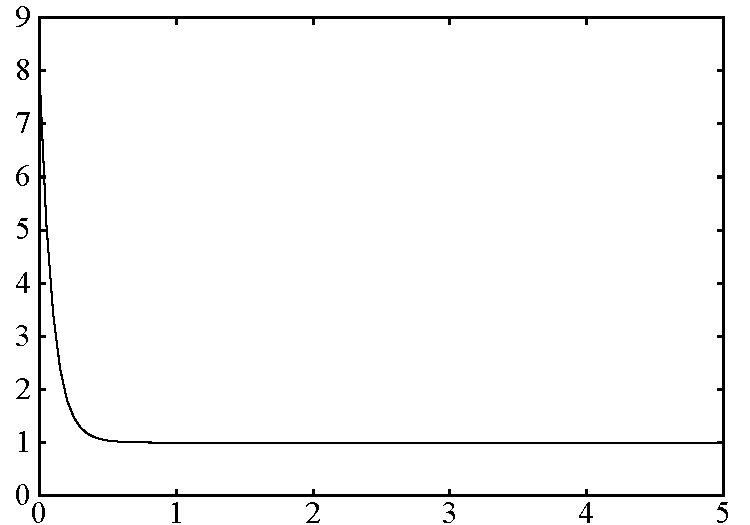
\includegraphics[height=60\unitlength]{apes_div}}
\cell{60}{-4}{b}{Viewpoint parameter, $q$}
\cell{15}{30}{c}{\rotatebox{90}{Diversity, $D_q(\p)$}}
\end{picture}

\caption{Abundances and species diversity profile of the estimated global
  distribution $\p$ of great apes (Hominidae).  Population estimates are
  all for 2016, with human data from United Nations~\cite{UNDE}, Tapanuli
  orangutan data from Nater et al.~\cite{Nate}, and all other data from the
  IUCN Red List of Threatened Species~\cite{AGMM,FHAF,HMOP,MBW,PRW,SWNU}.}  
\lbl{fig:apes}
\end{figure}

\begin{example}
\index{birds}
\lbl{eg:hill-birds}
% 
Figure~\ref{fig:bird-profs-bars} shows the diversity profiles of the 
two bird communities of the Introduction (p.~\pageref{p:intro-birds}).
% 
\begin{figure}
\lengths
\begin{picture}(61,50)(-5,-4)
\cell{28}{20}{c}{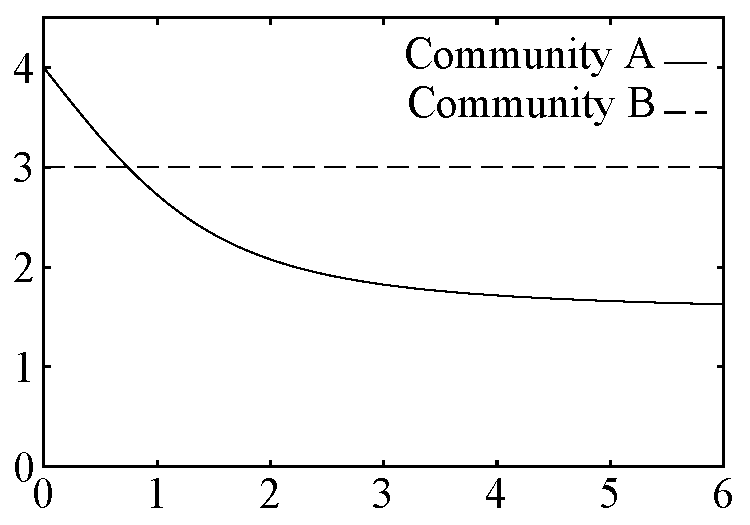
\includegraphics[height=40\unitlength]{AB.pdf}}
\put(30,30){\textcolor{white}{\rule{23.5\unitlength}{7.5\unitlength}}}
\cell{25}{15}{c}{Community A}
\cell{35}{30}{c}{Community B}
\cell{29}{-2}{c}{Viewpoint parameter, $q$}
\cell{-3}{21}{c}{\rotatebox{90}{Diversity, $D_q(\p)$}}
\end{picture}%
\hspace*{5mm}%
\lengths%
\begin{picture}(55,50)(-5,-4)
\cell{12}{24}{c}{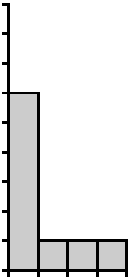
\includegraphics[width=20\unitlength]{birdbar1m}}
\cell{40}{24}{c}{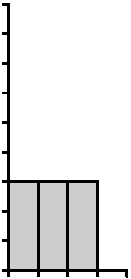
\includegraphics[width=20\unitlength]{birdbar2m}}
\cell{-3}{24}{c}{\rotatebox{90}{Probability}}
\cell{5.5}{2}{c}{$\scriptstyle 1$}
\cell{10}{2}{c}{$\scriptstyle 2$}
\cell{14.5}{2}{c}{$\scriptstyle 3$}
\cell{19}{2}{c}{$\scriptstyle 4$}
\cell{12}{-3}{b}{A}
\cell{1}{4}{c}{$\scriptstyle 0$}
\cell{1}{18}{c}{$\tfrac{1}{3}$}
\cell{1}{31}{c}{$\tfrac{2}{3}$}
\cell{1}{45}{c}{$\scriptstyle 1$}
% 
\cell{33.5}{2}{c}{$\scriptstyle 1$}
\cell{38}{2}{c}{$\scriptstyle 2$}
\cell{42.5}{2}{c}{$\scriptstyle 3$}
\cell{47}{2}{c}{$\scriptstyle 4$}
\cell{40}{-3}{b}{B}
\cell{29}{4}{c}{$\scriptstyle 0$}
\cell{29}{18}{c}{$\tfrac{1}{3}$}
\cell{29}{31}{c}{$\tfrac{2}{3}$}
\cell{29}{45}{c}{$\scriptstyle 1$}
\end{picture}
\caption{The diversity profiles of the two hypothetical bird communities in
  the Introduction (p.~\pageref{p:intro-birds}).}  
\lbl{fig:bird-profs-bars}
\end{figure}
% 
From the viewpoint%
%
\index{viewpoint!diversity@on diversity}
% 
of low values of $q$, where rare species are given
nearly as much importance as common species, community~A is more diverse
than community~B.  For instance, at $q = 0$, community~A is more diverse
than community~B simply because it has more species.  But from the
viewpoint of high values, which give less importance to rare species,
community~B seems more diverse because it is better balanced.  In the
extreme, when $q = \infty$, we ignore all species except the most common,
and the dominance of the first species in community~A makes that community
much less diverse than the well-balanced community~B.

The flat profile of community~B indicates the uniformity of the species
present.  Generally, we have seen in the last two examples that the shape
of a diversity profile provides information on the community's structure.
For more on the interpretation of diversity profiles, see Example~1,
Example~2 and Figure~2 of Leinster and Cobbold~\cite{MDISS}.%
%
\index{Cobbold, Christina}
\end{example}

\begin{example}
Diversity profiles arising from experimental data often cross one another
(as in the last example), indicating that different viewpoints%
%
\index{viewpoint!diversity@on diversity}
% 
on the importance of rare species lead to different judgements on which of
the communities is more diverse.  For example, Ellingsen tabulated
$D_0(\p)$, $D_1(\p)$ and $D_2(\p)$ for~16 distributions $\p$, corresponding
to the populations of certain marine organisms at~16 sites on the Norwegian
continental shelf (Table~1 of~\cite{Elli}).  There are $\binom{16}{2} =
120$ pairs of sites, and it can be deduced from the data that for at
least~$53$ of the~$120$ pairs, the profiles cross.

Typically, pairs of diversity profiles obtained from experimental data
cross at most once.  But it can be shown that in principle, there is no
upper bound on the number of times that a pair of diversity profiles can
cross. 
\end{example}


The ecological significance of the different judgements produced by
different diversity measures is discussed in the highly readable 1974 paper
of Peet~\cite{Peet}; see also Nagendra~\cite{Nage}.  More specifically,
diversity profiles of various types have long been discussed, beginning
with Hill%
%
\index{Hill Mark@Hill, Mark} 
%
himself in 1973~\cite{Hill}, and continuing with Patil%
%
\index{Patil, Ganapata P.} 
% 
and Taillie~\cite{PaTaSDP,PaTaDCM}, Dennis and Patil~\cite{DePa},
T\'othm\'er\'esz~\cite{TothCDM}, Patil~\cite{PatiDP}, Mendes et
al.~\cite{META}, and others.
% 
In political%
%
\index{politics}
% 
science, $D_q(\p)$ has been used as a measure of the effective%
%
\index{effective number!political parties@of political parties}
%
number of parties in a parliamentary assembly, and diversity profiles have
been used to compare the political situations of different countries at 
different times (Laakso and Taagepera~\cite{LaTa}, especially
equation~[8] and Figure~1).

The next section establishes the mathematical
properties of the Hill numbers and, therefore, of diversity profiles.


\section{Properties of the Hill numbers}
\lbl{sec:prop-hill}


Here we establish the main properties of the Hill numbers, using what we
already know about properties of the power means.  Of course, any statement
about the Hill numbers can be translated into a statement about R\'enyi
entropies, since one is the logarithm of the other.  But here we work with
the Hill numbers, interpreting them in terms of diversity.

We have already noted that for each $q \in [-\infty, \infty]$, the Hill
number $D_q$ is an effective number: $D_q(\vc{u}_n) = n$.

Diversity profiles are always decreasing.  Intuitively, this is because
diversity decreases as less importance is attached to rare species.  The
precise statement is as follows.

\begin{propn}
\lbl{propn:div-dec}
\index{Hill number!monotonicity in order}
\index{diversity profile!decreasing@is decreasing}
% 
Let $\p \in \Delta_n$.  Then $D_q(\p)$ is a decreasing function of $q \in
[-\infty, \infty]$.  It is constant if $\p$ is uniform on its support, and
strictly decreasing otherwise.
\end{propn}

\begin{proof}
Since $D_q(\p) = M_{1 - q}(\p, 1/\p)$, this follows from
Theorem~\ref{thm:mns-inc-ord}. 
\end{proof}

Figure~\ref{fig:bird-profs-bars} shows one strictly decreasing profile and one
that is constant (being uniform on its support).  Diversity profiles are
always continuous, by Lemma~\ref{lemma:pwr-mns-cts-t}.  

\begin{remark}
\lbl{rmk:prof-shapes}
\index{diversity profile!non-convex}
% 
It is a curiosity that for most distributions $\p$ that arise
experimentally, the diversity profile of $\p$ appears to be convex.  (See
the works cited at the end of Section~\ref{sec:ren-hill}, for example.)
However, this is false for arbitrary $\p$.  
Figure~\ref{fig:prof-not-cvx} shows the diversity profile of the
distribution
\[
\p = 
\bigl(
\underbrace{10^{-6}, \ldots, 10^{-6}}_{999\,000}, 10^{-3}
\bigr)
\]
(adapted from an example of Willerton~\cite{WillITG}),%
%
\index{Willerton, Simon} 
% 
which is evidently not convex.
% 
\begin{figure}
\centering
\lengths
\begin{picture}(120,60)(0,-5)
\cell{60}{27}{c}{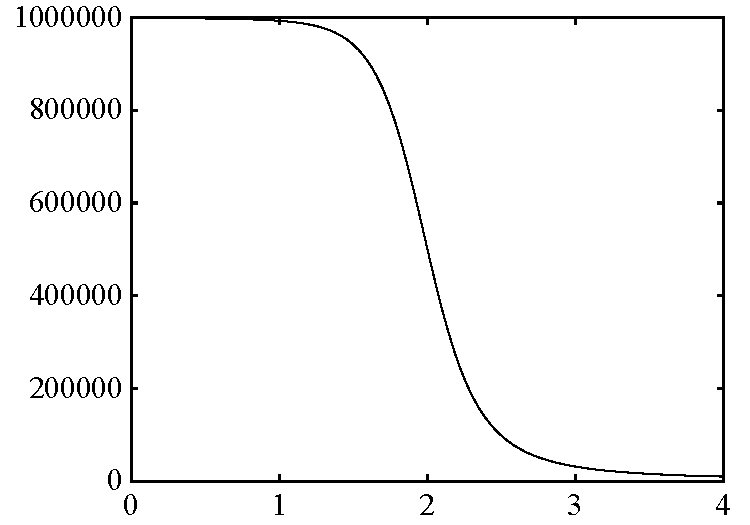
\includegraphics[width=80\unitlength]{noncon}}
\cell{66}{-5}{b}{$q$}
\cell{15}{28}{c}{$D_q(\p)$}
\end{picture}
\caption{A non-convex diversity profile (Remark~\ref{rmk:prof-shapes}).}
\lbl{fig:prof-not-cvx}
\end{figure}
\end{remark}

For each parameter value $q > 0$, the maximum and minimum values of the
Hill number $D_q$, and the distributions at which they are attained, are
exactly the same as for the diversity $D_1 = D$ of order~$1$
(Lemma~\ref{lemma:div1-max-min}):

\begin{lemma}
\lbl{lemma:div-max-min}
\index{Hill number!bounds on}
% 
Let $n \geq 1$ and $q \in [-\infty, \infty]$.
% 
\begin{enumerate}
\item 
\lbl{part:div-min}
$D_q(\p) \geq 1$ for all $\p \in \Delta_n$, with equality if and only if
$p_i = 1$ for some $i \in \{1, \ldots, n\}$.

\item
\lbl{part:div-max}
If $q > 0$ then $D_q(\p) \leq n$ for all $\p \in \Delta_n$, with
equality if and only if $\p = \vc{u}_n$.
\end{enumerate}
\end{lemma}

\begin{proof}
For~\bref{part:div-min}, Proposition~\ref{propn:div-dec} implies that
\[
D_q(\p)
\geq
D_{\infty}(\p)
=
1\Big/\!\!\max_{i \in \supp(\p)} p_i 
\geq 
1.
\]
If the second inequality is an equality then $p_i = 1$ for some $i$.
Conversely, if $p_i = 1$ for some $i$ then $D_q(\p) = 1$.

For~\bref{part:div-max}, Proposition~\ref{propn:div-dec} implies that
\[
D_q(\p)
\leq 
D_0(\p)
=
|\supp(\p)|
\leq 
n,
\]
with equality in the first inequality if and only if $\p$ is uniform on its
support.  On the other hand, equality holds in the second inequality if and
only if $\p$ has full support.  Hence equality holds throughout if and only
if $\p = \vc{u}_n$.
\end{proof}

\begin{remarks}
\lbl{rmks:hill-dec}
\begin{enumerate}
\item 
\lbl{rmk:hill-dec-min}
It follows that for $q > 0$, the R\'enyi entropy $H_q(\p)$ is minimized
exactly when $\p$ is of the form $(0, \ldots, 0, 1, 0, \ldots, 0)$, with
value $0$, and maximized exactly when $\p = \vc{u}_n$, with value $\log n$.
Since the $q$-logarithmic entropy $S_q(\p)$ is an increasing invertible
transformation of $H_q(\p)$ (equations~\eqref{eq:q-log-ren-slick}
and~\eqref{eq:ren-q-log-slick}), it is minimized and maximized at these same
distributions, with minimum $0$ and maximum $ S_q(\vc{u}_n) = \ln_q(n)$.

\item
\lbl{rmk:hill-dec-neg}
\index{Hill number!negative order@of negative order}
\index{order!negative}
% 
The Hill numbers of negative orders are \emph{not} maximized by the uniform
distribution.  Indeed, let $q < 0$, let $n \geq 2$, and take any non-uniform
distribution $\p \in \Delta_n$ of full support.
Then $D_0(\p) = |\supp(\p)| = n$, and the diversity profile of $\p$ is
strictly decreasing by Proposition~\ref{propn:div-dec}, so
\[
D_q(\p) > D_0(\p) = n = D_q(\vc{u}_n).
\]
Whatever the word `diverse' should mean, it is generally agreed that the
most diverse abundance distribution on a given set of species should be the
uniform distribution.  (At least, this should be the case for the crude
model of a community as a probability distribution, which we are using
here.  See also Section~\ref{sec:max}.)  For this reason, the Hill numbers
of negative orders are generally not used as measures of diversity.

On the other hand, the Hill numbers of negative orders measure
\emph{something}.  For instance, 
\[
D_{-\infty}(\p) = 1\Big/\!\min_{i \in \supp(\p)} p_i
= \max_{i \in \supp(\p)} (1/p_i)
\]
measures the rarity of the rarest species, giving a high value to any
community containing at least one species that is very rare.  This is a
meaningful quantity, even if it should not be called diversity.
\end{enumerate}
\end{remarks}

We now show that the Hill number $D_q(\p)$ of a given order $q$ is very
nearly continuous in $\p \in \Delta_n$, with the sole exception that $D_q$
is discontinuous at the boundary of the simplex when $q \leq 0$.  For
instance, species richness%
%
\index{species!richness} 
% 
$D_0$ is discontinuous: in terms of the number of species present, a
relative abundance of $0.0001$ is qualitatively different from a relative
abundance of $0$.

\begin{defn}
\lbl{defn:hill-cts}
Let $\bigl(D\from \Delta_n \to (0, \infty)\bigr)_{n \geq 1}$ be a sequence
of functions.  Then $D$ is 
\demph{continuous}%
%
\index{continuous!diversity measure} 
% 
if the function $D \from \Delta_n \to (0, \infty)$ is continuous for each
$n \geq 1$, and \demph{continuous% 
% 
\index{continuous!positive probabilities@in positive probabilities} 
% 
in positive probabilities} if the restriction $D|_{\Delta_n^\circ}$ of $D$
to the open simplex is continuous for each $n \geq 1$.
\end{defn}

Continuity in positive probabilities means that small changes to the
abundances of the species \emph{present} cause only small changes in the
perceived diversity.  For example, $D_0$ is continuous in positive
probabilities, even though it is not continuous.

\begin{lemma}
\lbl{lemma:hill-cts}
\index{Hill number!continuity of}
% 
\begin{enumerate}
\item 
\lbl{part:hill-cts-int}
For each $q \in [-\infty, \infty]$, the Hill number $D_q$ is continuous in
positive probabilities.

\item
\lbl{part:hill-cts-pos} 
For each $q \in (0, \infty]$, the Hill number $D_q$ is continuous.
\end{enumerate}
\end{lemma}

\begin{proof}
Part~\bref{part:hill-cts-int} is immediate from the explicit formulas for
$D_q$ (equations \eqref{eq:hill-gen}--\eqref{eq:hill-pinfty}), and
part~\bref{part:hill-cts-pos} follows from the observation that when $q >
0$, the formulas for $D_q$ are unchanged if we allow $i$ to range over all
of $\{1, \ldots, n\}$ instead of just $\supp(\p)$.
\end{proof}

Next we establish the algebraic properties of the Hill numbers, beginning
with the most elementary ones.  

\begin{defn}
\lbl{defn:hill-abs}
A sequence of functions $\bigl(D\from \Delta_n \to (0, \infty)\bigr)_{n
  \geq 1}$ is \demph{absence-invariant}%
%
\index{absence-invariance!diversity measure@of diversity measure} 
% 
if whenever $\p \in \Delta_n$ and $1 \leq i \leq n$ with $p_i = 0$, then
\[
D(\p) = D(p_1, \ldots, p_{i - 1}, p_{i + 1}, \ldots, p_n).
\]
\end{defn}

Absence-invariance means that as far as $D$ is concerned, a species that
is absent might as well not have been mentioned.  

Recall from equation~\eqref{eq:q-ent-sym} that $D$ is said to be
symmetric if $D(\p\sigma) = D(\p)$ for all $\p \in \Delta_n$ and
permutations $\sigma$ of $\{1, \ldots, n\}$.  This means that the
diversity is unaffected by the order in which the species happen to be
listed.

\begin{lemma}
\lbl{lemma:hill-elem}
\index{Hill number!symmetry of}
\index{Hill number!absence-invariance of}
% 
For each $q \in [-\infty, \infty]$, the Hill number $D_q$ of order $q$ is
symmetric and absence-invariant.
\end{lemma}

\begin{proof}
These statements follow from the symmetry and absence-invariance of the
power means (Lemma~\ref{lemma:pwr-mns-elem}).  Alternatively, they can be
deduced directly from the explicit formulas for $D_q$
(equations~\eqref{eq:hill-gen}--\eqref{eq:hill-pinfty}).
\end{proof}

\begin{remark}
\lbl{rmk:prof-perm}
\index{diversity profile!determines distribution}
% 
By symmetry, $\p$ and $\p\sigma$ have the same diversity profile.  In fact,
the converse also holds: if $\p, \vc{r} \in \Delta_n$ have the same
diversity profile then $\p$ and $\vc{r}$ must be the same up to a
permutation.  This is proved in Appendix~\ref{sec:prof}.

Thus, the diversity profile of a relative abundance distribution contains
all the information about that distribution apart from which species is
which, packaged in a way that displays meaningful information about the
community's diversity.
\end{remark}

We finally come to the chain rule.  In Corollary~\ref{cor:div1-chain}, we
treated the case $q = 1$, showing that
\[
D_1\bigl(\vc{w} \of (\p^1, \ldots, \p^n)\bigr)
=
D_1(\vc{w}) \cdot \prod_{i = 1}^n D_1(\p^i)^{w_i}
\]
for all $\vc{w} \in \Delta_n$ and $\p^i \in \Delta_{k_i}$.  In
Example~\ref{eg:div1-chain-islands}, this formula was explained in terms of
a group of $n$ islands of relative sizes $w_i$ and diversities $d_i =
D_1(\p^i)$, with no shared species.  We now give the chain rule for general
$q$, in two different forms.

\begin{propn}[Chain rule, version~1]
\lbl{propn:hill-chn}%
\index{chain rule!Hill numbers@for Hill numbers}%
\index{Hill number!chain rule for}
% 
Let $q \in [-\infty, \infty]$, $\vc{w} \in \Delta_n$, and $\p^1 \in
\Delta_{k_1}, \ldots, \p^n \in \Delta_{k_n}$.  Write $d_i = D_q(\p^i)$ and
$\vc{d} = (d_1, \ldots, d_n)$.  Then
% 
\begin{align*}
D_q\bigl(\vc{w} \of (\p^1, \ldots, \p^n)\bigr)  &
=
M_{1 - q}(\vc{w}, \vc{d}/\vc{w})        \\
&
=
\begin{cases}
\bigl(\sum w_i^q d_i^{1 - q}\bigr)^{1/(1 - q)}    &
\text{if } q \neq 1, \pm\infty, \\
\max d_i/w_i    &
\text{if } q = -\infty, \\
\prod (d_i/w_i)^{w_i}   &
\text{if } q = 1,       \\
\min d_i/w_i    &
\text{if } q = \infty, 
\end{cases}
\end{align*}
% 
where the sum, maximum, product, and minimum are over $i \in
\supp(\vc{w})$. 
\end{propn}

Here $\vc{d}/\vc{w} = (d_1/w_1, \ldots, d_n/w_n)$, as in
Remark~\ref{rmk:vec-op-conv}. 

\begin{proof}
We have
% 
\begin{align*}
D_q\bigl(\vc{w} \of (\p^1, \ldots, \p^n)\bigr)  &
=
M_{1 - q}\Bigl(\vc{w} \of (\p^1, \ldots, \p^n), 
\tfrac{1}{w_1 \p^1} \oplus\cdots\oplus \tfrac{1}{w_n \p^n} \Bigr)       \\
&
=
M_{1 - q}\Bigl(\vc{w},
\Bigl( 
M_{1 - q}\Bigl(\p^1, \tfrac{1}{w_1 \p^1}\Bigr), \,\ldots,\,
M_{1 - q}\Bigl(\p^n, \tfrac{1}{w_n \p^n}\Bigl)    
\Bigr)
\Bigr) \\
&
=
M_{1 - q}\bigl( \vc{w}, (d_1/w_1, \ldots, d_n/w_n) \bigr),
\end{align*}
% 
where the second equation follows from the chain rule for $M_{1 - q}$
(Proposition~\ref{propn:pwr-mns-chn}) and the last from the homogeneity of $M_{1
- q}$ (Lemma~\ref{lemma:pwr-mns-hgs}).  This proves the first equality
stated in the proposition, and the second follows from the explicit
formulas for the power means.
\end{proof}

There is an alternative form of the chain rule, for which we will need some
terminology.  Given a probability distribution $\vc{w} \in \Delta_n$ and a
real number $q$, the
\demph{escort%
%
\index{escort distribution}
%
distribution of order%
%
\index{order!escort distribution@of escort distribution} 
% 
$q$} of $\vc{w}$ is the distribution \ntn{wq}$\vc{w}^{(q)} \in \Delta_n$
with $i$th coordinate
\[
w^{(q)}_i
=
\begin{cases}
w_i^q \bigg/\!\!\sum\limits_{j \in \supp(\vc{w})} w_j^q &
\text{if } i \in \supp(\vc{w}),     \\
0       &
\text{otherwise}.
\end{cases}
\]

\begin{lemma}
\lbl{lemma:mean-esc}
Let $q \in \R$, $\vc{w} \in \Delta_n$, and $\vc{d} \in [0, \infty)^n$.
Then
\[
M_{1 - q}(\vc{w}, \vc{d}/\vc{w})
=
D_q(\vc{w}) \cdot M_{1 - q}(\vc{w}^{(q)}, \vc{d}).
\]
\end{lemma}

\begin{proof}
For the case $q = 1$, note that
\[
M_0(\vc{w}, \vc{x}\vc{y}) =
M_0(\vc{w}, \vc{x}) M_0(\vc{w}, \vc{y})
\]
for all $\vc{x}, \vc{y} \in [0, \infty)^n$.  It follows that
\[
D_1(\vc{w}) \cdot M_0(\vc{w}^{(1)}, \vc{d})
=
M_0(\vc{w}, 1/\vc{w}) \cdot M_0(\vc{w}, \vc{d})
=
M_0(\vc{w}, \vc{d}/\vc{w}).
\]
On the other hand, for $1 \neq q \in \R$,
% 
\begin{align*}  
M_{1 - q}(\vc{w}, \vc{d}/\vc{w})        &
=
\Biggl( \sum_{i \in \supp(\vc{w})} w_i^q d_i^{1 - q} \Biggr)^{1/(1 - q)}\\
&
=
D_q(\vc{w}) \cdot
\Biggl( 
\frac{\sum_{i \in \supp(\vc{w})} w_i^q d_i^{1 - q}}%
{\sum_{j \in \supp(\vc{w})} w_j^q}
\Biggr)^{1/(1 - q)}       \\
&
=
D_q(\vc{w}) \cdot M_{1 - q}(\vc{w}^{(q)}, \vc{d}),
\end{align*}
% 
as required.
\end{proof}

The last two results immediately imply:

\begin{propn}[Chain rule, version~2]
\lbl{propn:hill-chn-esc}%
\index{chain rule!Hill numbers@for Hill numbers}%
\index{Hill number!chain rule for}
% 
Let $q \in \R$, $\vc{w} \in \Delta_n$, and $\p^1 \in
\Delta_{k_1}, \ldots, \p^n \in \Delta_{k_n}$.  Write $d_i = D_q(\p^i)$ and 
$\vc{d} = (d_1, \ldots, d_n)$.  Then
\[
D_q\bigl(\vc{w} \of (\p^1, \ldots, \p^n)\bigr)
=
D_q(\vc{w}) \cdot M_{1 - q}(\vc{w}^{(q)}, \vc{d}).
\]
\qed
\end{propn}

\begin{remarks}
\lbl{rmks:hill-chn}
Here we provide context for the notion of escort distribution.
% 
\begin{enumerate}
\item
The escort distributions of a distribution $\vc{w}$ form a 
one-parameter family
\[
\bigl( \vc{w}^{(q)} \bigr)_{q \in \R}
\]
of distributions, of which the original distribution $\vc{w}$ is the member
corresponding to $q = 1$.  The term `escort distribution' is taken from
thermodynamics\index{thermodynamics} (Chapter~9 of Beck and
Schl\"ogl~\cite{BeSc}).  There, one encounters expressions such as
\[
\frac{(e^{-\beta E_1}, \ldots, e^{-\beta E_n})}{Z(\beta)},
\]
where $Z(\beta) = e^{-\beta E_1} + \cdots + e^{-\beta E_n}$ is the
partition%
%
\index{partition function} 
%
function for energies $E_i$ at inverse temperature $\beta$.
Assuming without loss of generality that $\sum e^{-E_i} = 1$, the inverse
temperature $\beta$ plays the role of the parameter $q$.

\item
\lbl{rmk:hill-chn-vs}
The function $(q, \vc{w}) \mapsto \vc{w}^{(q)}$ is the scalar
multiplication of a real vector space structure on the interior
$\Delta_n^\circ$ of the simplex.%
%
\index{simplex!vector space structure on}
% 
Addition is given by 
\[
(\vc{p}, \vc{r}) 
\mapsto
\frac{(p_1 r_1, \ldots, p_n r_n)}{p_1 r_1 + \cdots + p_n r_n},
\]
and the zero element is the uniform distribution $\vc{u}_n$.
Figure~\ref{fig:simp-vs} shows some one-dimensional linear subspaces of the
two-dimensional vector space $\Delta_3^\circ$.
% 
\begin{figure}
\centering
\lengths
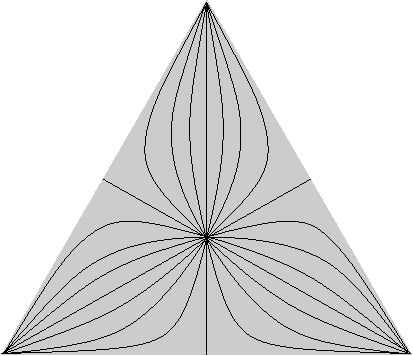
\includegraphics[width=70\unitlength]{subspaces_quietm}
\caption{Twelve one-dimensional linear subspaces of the open simplex
  $\Delta_3^\circ$ with the real vector space structure described in
  Remark~\ref{rmks:hill-chn}\bref{rmk:hill-chn-vs}.}
\lbl{fig:simp-vs}
\end{figure}
% 
This vector space structure was used in the field of statistical inference
by Aitchison~\cite{Aitc},%
%
\index{Aitchison, John} 
% 
and is sometimes named after him.  It can be understood algebraically as
follows.

Exponential and logarithm define a bijection between $\R$ and $(0,
\infty)$.  This induces a bijection between $\R^n$ and $(0, \infty)^n$, and
transporting the vector space structure on $\R^n$ across this bijection
gives a vector space structure on $(0, \infty)^n$.  Explicitly, addition in
the vector space $(0, \infty)^n$ is coordinatewise multiplication, the zero
element is $(1, \ldots, 1)$, and scalar multiplication by $q \in \R$ raises
each coordinate to the power of $q$.

Now take the linear subspace of $\R^n$ spanned by $(1, \ldots, 1)$.  The
corresponding subspace $W$ of $(0, \infty)^n$ is $\{ (\gamma, \ldots,
\gamma) \such \gamma \in (0, \infty) \}$, and we can form the quotient
vector space $(0, \infty)^n/W$.

An element of this quotient is an equivalence class of vectors $\vc{y} \in
(0, \infty)^n$, with $\vc{y}$ equivalent to $\vc{z}$ if and only if $\vc{y}
= \gamma\vc{z}$ for some $\gamma > 0$.  Geometrically, then, the
equivalence classes are the rays through the origin in the positive orthant
$(0, \infty)^n$.  Each ray contains exactly one element of the open simplex
\[
\Delta_n^\circ
=
\{ \vc{y} \in (0, \infty)^n \such y_1 + \cdots + y_n = 1 \}.
\]
This puts $(0, \infty)^n/W$ in bijection with $\Delta_n^\circ$, thus giving
$\Delta_n^\circ$ the structure of a vector space.  It is exactly the
vector space structure defined explicitly above.

\item
In statistical language, each linear subspace of the vector space
$\Delta_n^\circ$ is an exponential%
%
\index{exponential family} 
% 
family of distributions on $\{1, \ldots, n\}$.  For example, the
one-dimensional subspace spanned by $\p \in \Delta_n^\circ$ is a
one-parameter exponential family with natural parameter $q \in \R$,
sufficient statistic $\log p_i$, and log-partition%
%
\index{partition function}
%
function $\log\bigl(\sum p_i^q\bigr)$.  More on this connection
can be found in Amari~\cite{AmarDGC}, Ay, Jost, L\^{e} and
Schwachh\"ofer (\cite{AJLS}, Section~2.8), and other information%
%
\index{information geometry}
%
geometry texts.
\end{enumerate}
\end{remarks}

As already discussed in the case $q = 1$
(Example~\ref{eg:div1-chain-islands}), the chain rule for the Hill numbers
has the important consequence that when computing the total diversity of a
group of islands%
%
\index{islands!diversity of group of} 
% 
with no shared species, the only information one needs is the diversities
and relative sizes of the islands, not their internal make-up:

\begin{defn}
\lbl{defn:hill-mod}
A sequence of functions $\bigl(D \from \Delta_n \to (0, \infty) \bigr)_{n
  \geq 1}$ is \demph{modular}%
%
\index{modularity!diversity measure@of diversity measure}
%
if 
% 
\begin{align*}
&
D\bigl(\p^i\bigr) = D\bigl(\twid{\p}^i\bigr) 
\text{ for all } i \in \{1, \ldots, n\}     \\
\implies
&
D\bigl( \vc{w} \of (\p^1, \ldots, \p^n) \bigr) =
D\bigl( \vc{w} \of (\twid{\p}^1, \ldots, \twid{\p}^n) \bigr) 
\end{align*}
% 
for all $n, k_1, \ldots, k_n, \twid{k}_1, \ldots, \twid{k}_n \geq 1$ and
$\vc{w} \in \Delta_n$, $\p^i \in \Delta_{k_i}$, $\twid{\p}^i \in
\Delta_{\twid{k}_i}$.  
\end{defn}

In other words, $D$ is modular if $D\bigl( \vc{w} \of (\p^1, \ldots, \p^n)
\bigr)$ depends only on $\vc{w}$ and $D(\p^1), \ldots, D(\p^n)$. 

\begin{cor}[Modularity]
\lbl{cor:mod-hill}
\index{Hill number!modularity of}%
\index{modularity!Hill numbers@of Hill numbers}
% 
For each $q \in [-\infty, \infty]$, the Hill number $D_q$ is modular.
\qed
\end{cor}

The chain rule has two further consequences.

\begin{defn}
\lbl{defn:hill-mult}
A sequence of functions $\bigl( D \from \Delta_n \to (0, \infty) \bigr)_{n
  \geq 1}$ is \demph{multiplicative}%
%
\index{multiplicative!diversity measure} 
% 
if 
\[
D(\p \otimes \vc{r}) = D(\p) D(\vc{r})
\]
for all $m, n \geq 1$, $\p \in \Delta_m$, and $\vc{r} \in \Delta_n$. 
\end{defn}

\begin{cor}[Multiplicativity]
\index{Hill number!multiplicativity of}%
\index{multiplicative!Hill numbers are}
% 
For each $q \in [-\infty, \infty]$, the Hill number $D_q$ is
multiplicative. 
\end{cor}

\begin{proof}
This follows from either 
the chain rule for the Hill numbers
or the logarithmic property of the
R\'enyi entropies (equation~\eqref{eq:ren-log}).
\end{proof}

\begin{defn}
\lbl{defn:hill-rep}
A sequence of functions $\bigl( D \from \Delta_n \to (0, \infty) \bigr)_{n
  \geq 1}$ satisfies the 
\demph{replication%
%
\index{replication principle} 
% 
principle} if 
\[
D(\vc{u}_n \otimes \p) = nD(\p)
\]
for all $n, k \geq 1$ and $\p \in \Delta_k$.
\end{defn}

The oil company argument of Example~\ref{eg:oil} shows the fundamental
importance of the replication principle.  If $n$ islands have the same
relative abundance distribution $\p$, but on disjoint sets of species, the
diversity of the whole system should be $nD(\p)$.

\begin{cor}[Replication]
\index{Hill number!replication principle for}
\index{replication principle!Hill numbers@for Hill numbers}
% 
For each $q \in [-\infty, \infty]$, the Hill number $D_q$ satisfies the
replication principle.
\end{cor}

\begin{proof}
This follows from multiplicativity and the fact that $D_q$ is an effective
number. 
\end{proof}

Accompanying the R\'enyi entropies, there is also a notion of R\'enyi
relative entropy (introduced in Section~3 of R\'enyi~\cite{Reny}).  We
defer discussion to Section~\ref{sec:value-rel}.


\section{Characterization of the Hill number of a given order}
\lbl{sec:hill-char-given}
\index{Hill number!characterization of}


In this book, we prove two characterization theorems for the Hill numbers.
The first states that for each given $q$, the unique function satisfying
certain conditions (which depend on $q$) is $D_q$.  The second states that
the only functions satisfying a different list of conditions (which make no
mention of $q$) are those belonging to the family $(D_q)_{q \in [-\infty,
    \infty]}$.  We prove the first characterization in this section, and
the second in Section~\ref{sec:total-hill}.

For the $q$-logarithmic entropies, we have already proved an analogue of
the first result (Theorem~\ref{thm:q-ent-char}).  We will not prove an
analogue of the second.  However, there is a theorem of this type due to
Forte and Ng, briefly discussed in Remark~\ref{rmk:total-hill-translate}.

Here we build on work of Routledge~\cite{Rout} to characterize the Hill
number $D_q$ for each given $q \in (0, \infty)$.  The restriction to positive
$q$ ensures that $D_q$ is continuous on all of $\Delta_n$ (by
Lemma~\ref{lemma:hill-cts}\bref{part:hill-cts-pos}).  

Recall that $D_q$ satisfies the chain rule
% 
\begin{equation}
\lbl{eq:hill-chn-esc-char}
D_q \bigl( \vc{w} \of (\p^1, \ldots, \p^n) \bigr)
=
D_q(\vc{w}) \cdot
M_{1 - q} \Bigl(
\vc{w}^{(q)}, \bigl(D_q(\p^1), \ldots, D_q(\p^n)\bigr)
\Bigr),
\end{equation}
% 
where $\vc{w} \in \Delta_n$ and $\p^i \in \Delta_{k_i}$
(Proposition~\ref{propn:hill-chn-esc}).
% 
Let us reflect on equation~\eqref{eq:hill-chn-esc-char}, interpreting it in
terms of the island%
%
\index{islands!diversity of group of} 
% 
scenario of Examples~\ref{eg:comp-islands} and~\ref{eg:div1-chain-islands}.
Equation~\eqref{eq:hill-chn-esc-char} can be interpreted as a decomposition
of the diversity of the island group into two factors: the variation
\emph{between} the islands (given by $D_q(\vc{w})$), and the average
variation or diversity \emph{within} the islands (given by the second
factor).  Recall that in the island scenario, there is no overlap of
species between islands, so the variation between the islands depends only
on the variation in sizes.

Now, suppose that we want to list some properties that a reasonable
diversity measure $D$ ought to satisfy.  One such property might be that
$D$ is decomposable in the sense just described: $D(\vc{w} \of (\p^1,
\ldots, \p^n))$ is equal to the variation $D(\vc{w})$ between islands
multiplied by the average of the diversities $D(\p^1), \ldots, D(\p^n)$
within each island.

But what could `average' reasonably mean?  We have already seen that the
power means have many good properties that we would expect of a notion of
avarage, and we will see in Chapter~\ref{ch:mns} that in a certain precise
sense, they are \emph{uniquely} good.  So, it is reasonable to take the
`average' to be some power mean $M_t$, and we can make the usual harmless
reparametrization $t = 1 - q$.

This reasoning suggests that our hypothetical diversity measure $D$ should
satisfy something like equation~\eqref{eq:hill-chn-esc-char}, with $D$ in
place of $D_q$.  Still, it does not explain why the average of the
within-island diversities should be calculated using the weighting
$\vc{w}^{(q)}$ on the islands, 
rather than some other weighting.  All that seems
clear is that the weighting should depend on the sizes of the islands only.
If we write the weighting as $\theta(\vc{w})$, then our conclusion is that
any reasonable diversity measure $D$ ought to satisfy the equation
\[
D \bigl( \vc{w} \of (\p^1, \ldots, \p^n) \bigr)
=
D(\vc{w}) \cdot
M_{1 - q} \Bigl(
\theta(\vc{w}), \bigl(D(\p^1), \ldots, D(\p^n)\bigr)
\Bigr)
\]
for some $q$ and some function $\theta \from \Delta_n \to \Delta_n$.  This
explains the most substantial of the hypotheses in our main result:

\begin{thm}
\lbl{thm:rout}
\index{Hill number!characterization of}
% 
Let $q \in (0, \infty)$.  Let $\bigl( D \from \Delta_n \to (0, \infty)
\bigr)_{n \geq 1}$ be a sequence of functions.  The following are
equivalent: 
% 
\begin{enumerate}
\item
\lbl{part:rout-condns}
the functions $D$ are continuous, symmetric and effective numbers, and for
each $n \geq 1$ there exists a function $\theta \from \Delta_n \to
\Delta_n$ with the following property: 
\[
D \bigl( \vc{w} \of (\p^1, \ldots, \p^n) \bigr)
=
D(\vc{w}) \cdot
M_{1 - q} \Bigl(
\theta(\vc{w}), \bigl(D(\p^1), \ldots, D(\p^n)\bigr)
\Bigr)
\]
for all $\vc{w} \in \Delta_n$, $k_1, \ldots, k_n \geq 1$, and $\p^i \in
\Delta_{k_i}$;

\item
\lbl{part:rout-form}
$D = D_q$.
\end{enumerate}
\end{thm}

Theorem~\ref{thm:rout} is a variation on a 1979 result of
Routledge%
%
\index{Routledge, Richard}
%
(Theorem~1 of the appendix to \cite{Rout}).

The rest of this section is devoted to the proof.  We already showed in
Section~\ref{sec:prop-hill} that~\bref{part:rout-form}
implies~\bref{part:rout-condns}.  Conversely, and \femph{for the rest of
  this section}, take $D$ and $\theta$ satisfying the conditions
of~\bref{part:rout-condns}.  By the standard abuse of notation, we use the
same letter $\theta$ for each of the functions $\theta \from \Delta_1 \to
\Delta_1$, $\theta \from \Delta_2 \to \Delta_2$, etc.  We have to prove
that $D = D_q$.

For $\p \in \Delta_n$, write
\[
\theta(\p) = \bigl( \theta_1(\p), \ldots, \theta_n(\p) \bigr).
\]
Our first lemma shows how $\theta_1$ can be expressed in terms of $D$.  We
temporarily adopt the notation
% 
\[
\splitdist{\p}  
=
\p \of (\vc{u}_2, \vc{u}_1, \ldots, \vc{u}_1)   
=
\bigl( \hlf p_1, \hlf p_1, p_2, \ldots, p_n \bigr)
\ntn{hash}
\]
($\p \in \Delta_n$).

\begin{lemma}
\lbl{lemma:rout-th1}
For all $n \geq 1$ and $\p \in \Delta_n$,
\[
\theta_1(\p)
=
\frac{1}{\ln_q 2} \cdot \ln_q \frac{D(\splitdist{\p})}{D(\p)}.
\]
\end{lemma}

\begin{proof}
By the main hypothesis on $D$ and the effective number property,
\[
D(\splitdist{\p}) 
=
D(\p) \cdot M_{1 - q}\bigl( \theta(\p), (2, 1, \ldots, 1) \bigr).
\]
Hence by Lemma~\ref{lemma:q-log-mean},
\[
\ln_q \frac{D(\splitdist{\p})}{D(\p)} 
=
M_1 \bigl( \theta(\p), (\ln_q 2, \ln_q 1, \ldots, \ln_q 1) \bigr).
\]
But $\ln_q 1 = 0$, so the right-hand side is just $\theta_1(\p) \ln_q 2$.
\end{proof}

We use this lemma to compute the weighting $\theta(\vc{w}\of(\p^1, \ldots,
\p^n))$ of a composite distribution:

\begin{lemma}
\lbl{lemma:rout-theta-comp}
Let $\vc{w} \in \Delta_n$ and $\p^1 \in \Delta_{k_1}, \ldots, \p^n \in
\Delta_{k_n}$.  Then
\[
\theta_1\bigl( \vc{w} \of (\p^1, \ldots, \p^n) \bigr)
=
\frac{\theta_1(\vc{w}) D(\p^1)^{1 - q}}%
{\sum_{i = 1}^n \theta_i(\vc{w}) D(\p^i)^{1 - q}}
\,
\theta_1(\p^1).
\]
\end{lemma}

\begin{proof}
Write $d_i = D(\p^i)$ and $\spltdist{d_1} = D\Bigl(\splitdist{\p^1}\Bigr)$.
We have
% 
\begin{align}
&
\theta_1\bigl(\vc{w} \of (\p^1, \ldots, \p^n)\bigr)
\nonumber
\\
&
=
\frac{1}{\ln_q 2} \cdot 
\ln_q 
\frac{D \Bigl(\Splitdist{\vc{w} \of (\p^1, \ldots, \p^n)}\Bigr)}%
{D\bigl( \vc{w} \of (\p^1, \ldots, \p^n)\bigr)}  
\lbl{eq:rtc-1}  \\
&
=
\frac{1}{\ln_q 2} \cdot 
\ln_q 
\frac{D \Bigl(\vc{w} \of 
\Bigl( \splitdist{\p^1}, \p^2, \ldots, \p^n\Bigr)
\Bigr)}%
{D\bigl( \vc{w} \of (\p^1, \p^2, \ldots, \p^n)\bigr)}  
\lbl{eq:rtc-2}  \\
&
=
\frac{1}{\ln_q 2} \cdot 
\ln_q 
\frac{M_{1 - q} \bigl(\theta(\vc{w}),
(\spltdist{d_1}, d_2, \ldots, d_n)
\bigr)}%
{M_{1 - q} \bigl( \theta(\vc{w}), (d_1, d_2, \ldots, d_n)\bigr)}  
\lbl{eq:rtc-3}  \\
&
=
\frac{1}{\ln_q 2} \cdot 
\frac{%
\ln_q M_{1 - q}\bigl(\theta(\vc{w}), (\spltdist{d_1}, d_2, \ldots, d_n)\bigr)
-
\ln_q M_{1 - q}\bigl(\theta(\vc{w}), (d_1, d_2, \ldots, d_n)\bigr)
}%
{M_{1 - q} \bigl( \theta(\vc{w}), (d_1, d_2, \ldots, d_n)\bigr)^{1 - q}}  
\lbl{eq:rtc-4}  \\
&
=
\frac{1}{\ln_q 2} \cdot 
\frac{%
M_1\bigl(
\theta(\vc{w}), (\ln_q \spltdist{d_1}, \ln_q d_2, \ldots)
\bigr)
-
M_1\bigl(
\theta(\vc{w}), (\ln_q d_1, \ln_q d_2, \ldots)
\bigr)
}%
{\sum_{i = 1}^n \theta_i(\vc{w}) d_i^{1 - q}}
\lbl{eq:rtc-5}  \\
&
=
\frac{1}{\ln_q 2} \cdot
\frac{
\theta_1(\vc{w}) (\ln_q \spltdist{d_1} - \ln_q d_1)
}%
{\sum_{i = 1}^n \theta_i(\vc{w}) d_i^{1 - q}}
\lbl{eq:rtc-6}  \\
&
=
\frac{1}{\ln_q 2} \cdot
\frac{
\theta_1(\vc{w}) d_1^{1 - q}
}%
{\sum_{i = 1}^n \theta_i(\vc{w}) d_i^{1 - q}}
\cdot
\ln_q \frac{\spltdist{d_1}}{d_1} 
\lbl{eq:rtc-7}  \\
&
=
\frac{\theta_1(\vc{w}) d_1^{1 - q}}%
{\sum_{i = 1}^n \theta_i(\vc{w}) d_i^{1 - q}}
\cdot
\theta_1(\p^1)
\lbl{eq:rtc-8},
\end{align}
% 
where equations~\eqref{eq:rtc-1} and~\eqref{eq:rtc-8} follow from
Lemma~\ref{lemma:rout-th1}, equation~\eqref{eq:rtc-2} from the definition of
$\splitdist{\ }$, equation~\eqref{eq:rtc-3} from the main hypothesis on $D$,
equations~\eqref{eq:rtc-4} and~\eqref{eq:rtc-7} from the quotient formula
\[
\ln_q \frac{x}{y} 
=
\frac{\ln_q x - \ln_q y}{y^{1 - q}}
\]
for the $q$-logarithm (equation~\eqref{eq:q-log-qt}),
equation~\eqref{eq:rtc-5} from Lemma~\ref{lemma:q-log-mean} and the
definition of $M_{1 - q}$, and equation~\eqref{eq:rtc-6} from the
definition of the arithmetic mean $M_1$.
\end{proof}

We now deduce that the weightings must be the $q$-escort distributions:

\begin{lemma}
\lbl{lemma:rout-wts}
$\theta(\vc{w}) = \vc{w}^{(q)}$ for all $n \geq 1$ and $\vc{w} \in
  \Delta_n$. 
\end{lemma}

\begin{proof}
Following a familiar pattern, we prove this first when $\vc{w}$ is uniform,
then when the coordinates of $\vc{w}$ are positive and rational, and
finally for arbitrary $\vc{w}$.

For the case $\vc{w} = \vc{u}_n$, we have to prove that $\theta(\vc{u}_n) =
\vc{u}_n$.  By Lemma~\ref{lemma:rout-th1},
\[
\theta_1(\vc{u}_n)
=
\frac{1}{\ln_q 2}
\ln_q
\frac{D\bigl( 
\vc{u}_n \of (\vc{u}_2, \vc{u}_1, \vc{u}_1, \ldots, \vc{u}_1)
\bigr)}{D(\vc{u}_n)},
\]
and by the same argument,
\[
\theta_2(\vc{u}_n)
=
\frac{1}{\ln_q 2}
\ln_q
\frac{D\bigl( 
\vc{u}_n \of (\vc{u}_1, \vc{u}_2, \vc{u}_1, \ldots, \vc{u}_1)
\bigr)}{D(\vc{u}_n)}.
\]
By symmetry of $D$, the right-hand sides of these two equations are equal.
Hence $\theta_1(\vc{u}_n) = \theta_2(\vc{u}_n)$.  Similarly,
$\theta_i(\vc{u}_n) = \theta_j(\vc{u}_n)$ for all $i, j$, and so
$\theta(\vc{u}_n) = \vc{u}_n$. 

Now let $\vc{w} \in \Delta_n$ with 
\[
\vc{w} = (k_1/k, \ldots, k_n/k)
\]
for some positive integers $k_i$, where $k = \sum k_i$.  We have
% 
\begin{equation}
\lbl{eq:rout-rat}
\vc{w} \of (\vc{u}_{k_1}, \ldots, \vc{u}_{k_n})
=
\vc{u}_k.
\end{equation}
% 
Applying $\theta_1$ to both sides gives
\[
\frac{\theta_1(\vc{w}) k_1^{1 - q}}{\sum \theta_i(\vc{w}) k_i^{1 - q}}
\, \frac{1}{k_1}
=
\frac{1}{k},
\]
using Lemma~\ref{lemma:rout-theta-comp}, the effective number property of
$D$, and the previous paragraph.  This rearranges to
\[
\theta_1(\vc{w}) 
=
w_1^q \sum_{i = 1}^n \theta_i(\vc{w}) w_i^{1 - q}.
\]
By the same argument,
\[
\theta_j(\vc{w})
=
w_j^q \sum_{i = 1}^n \theta_i(\vc{w}) w_i^{1 - q}
\]
for all $j = 1, \ldots, n$.  The sum on the right-hand side is independent
of $j$, so $\theta(\vc{w})$ is a probability distribution proportional to
$\bigl(w_1^q, \ldots, w_n^q\bigr)$, forcing $\theta(\vc{w}) = \vc{w}^{(q)}$. 

Finally, we show that $\theta(\vc{w}) = \vc{w}^{(q)}$ for all $\vc{w} \in
\Delta_n$.  By Lemma~\ref{lemma:rout-th1} and the continuity hypothesis on
$D$, the map $\theta_1$ is continuous, and similarly for $\theta_2, \ldots,
\theta_n$.  Hence $\theta \from \Delta_n \to \Delta_n$ is continuous.  So
too is the map $\vc{w} \mapsto \vc{w}^{(q)}$.  But by the previous
paragraph, these last two maps are equal on the positive rational
distributions, so they are equal everywhere.
\end{proof}

\begin{pfof}{Theorem~\ref{thm:rout}}
First, consider distributions $\vc{w} = (k_1/k, \ldots, k_n/k)$ with
positive rational coordinates.  Apply $D$ to both sides of
equation~\eqref{eq:rout-rat}: then by Lemma~\ref{lemma:rout-wts} and the
effective number hypothesis on $D$,
\[
D(\vc{w}) \cdot M\bigl( \vc{w}^{(q)}, (k_1, \ldots, k_n ) \bigr)
=
k.
\]
But we can also apply $D_q$ to both sides of equation~\eqref{eq:rout-rat}:
then by the chain rule and the effective number property of $D_q$,
\[
D_q(\vc{w}) \cdot M\bigl( \vc{w}^{(q)}, (k_1, \ldots, k_n) \bigr)
=
k.
\]
Hence $D(\vc{w}) = D_q(\vc{w})$.  And by the continuity hypothesis on $D$
and the continuity property of $D_q$
(Lemma~\ref{lemma:hill-cts}\bref{part:hill-cts-pos}), it follows that
$D(\vc{w}) = D_q(\vc{w})$ for all $\vc{w} \in \Delta_n$.
\end{pfof}
